%%%%%%%%%%%%%%%%%%%%%%%%%%%%%%%%%%%%%%%%%%%%%%%%%%%%%%%%%%%%%%%%%%%%%%%
% Vorlage für Bachelor- und Masterarbeiten mit pdflatex nach dem Layout des ITS
% Fabian Bleier (fabian.bleier@kit.edu), September 2016
%%%%%%%%%%%%%%%%%%%%%%%%%%%%%%%%%%%%%%%%%%%%%%%%%%%%%%%%%%%%%%%%%%%%%%%
% Kurzbeschreibung
% Der Hauptordner enthält in erster Linie das Dokument "gesamt.tex". Dieses enthält wiederum alle notwendigen Nutzereingaben (Autor, Titel etc.). 
% Die einzelnen Kapitel werden in das Gesamtdokument eingeladen und liegen im Ordner "kapitel". 
% Der Ordner "sonstiges" enthält alle Seiten außerhalb des eigentlichen Textkörpers (Formatierung der Kopfzeilen, Deckblätter, die einzubindenden Pakete, Institutslogos, Macros, Verzeichnisse usw.)
% Der Ordner "literatur" enthält alle Dateien, welche zur Gestaltung eines Literaturverzeichnisses notwendig sind (Die bibtex-Datei, die bst-Datei, und das eigentliche Verzeichnis).
% Im Ordner "bilder" können alle Abbildungen abgelegt werden.
% Der Ordner "dokumentation" enthält verschiedene Dokumentationen zu den verwendeten Paketen, ferner eine ausbaufähige Dokumentation des LaTeX-Dokuments

%%%%%%%%%%%%%%%%%%%%%%%%%%%%%%%%%%%%%%%%%%%%%%%%%%%%%%%%%%%%%%%%%%%%%%%
% Dokumenterstellung
%%%%%%%%%%%%%%%%%%%%%%%%%%%%%%%%%%%%%%%%%%%%%%%%%%%%%%%%%%%%%%%%%%%%%%%
\documentclass[
paper=a4,										% Seitenformat
12pt,											% Schriftgröße
twoside=false,									% zweiseitig true/false
headings=small,									% Formatierung der Überschriften
draft=false,									% Entwurfsmodus true/false
]{scrreprt}										% KOMA-Klasse Report
%\usepackage{showframe}							% Schriftfeld in Dokument anzeigen

%%%%%%%%%%%%%%%%%%%%%%%%%%%%%%%%%%%%%%%%%%%%%%%%%%%%%%%%%%%%%%%%%%%%%%%
% Metadaten und Variablen zur Verwendung im Dokument und zur Erstellung der PDF-Datei
%%%%%%%%%%%%%%%%%%%%%%%%%%%%%%%%%%%%%%%%%%%%%%%%%%%%%%%%%%%%%%%%%%%%%%%
\newcommand{\doctitle}{Implementation of a Nearest-Neighbor Search for Particle Simulation in Sparse Computational Domains} 				% Titel der Arbeit
\newcommand{\doctype}{Energietechnisches Praktikum}			% Dokumenttyp
\newcommand{\docauthor}{Jens Peifle, B.Sc.}	% Autor
\newcommand{\doclocation}{Karlsruhe}			% Erstellungsort
\newcommand{\betreuerI}{Marc Keller, M.Sc.}	% Betreuer1
\newcommand{\betreuerII}{}						% Betreuer2 (optional, kann leer gelassen werden)
\newcommand{\docsubject}{Kurzbeschreibung}		% Kurzbeschreibung
\newcommand{\dockeywords}{%
Flugzeugtriebwerke,
	SPH, Partikel
}												% Stichworte
\newcommand{\doccreator}{pdflatex}				% Erstellt mit
\newcommand{\docproducer}{LaTeX}				% Software
\newcommand{\docdate}{\today}					% Erstellungsdatum

%%%%%%%%%%%%%%%%%%%%%%%%%%%%%%%%%%%%%%%%%%%%%%%%%%%%%%%%%%%%%%%%%%%%%%%
% Formatierung, Pakete, Makros einbinden
%%%%%%%%%%%%%%%%%%%%%%%%%%%%%%%%%%%%%%%%%%%%%%%%%%%%%%%%%%%%%%%%%%%%%%%
%%%%%%%%%%%%%%%%%%%%%%%%%%%%%%%%%%%%%%%%%%%%%%%%%%%%%%%%%%%%%%%%%%%%%%%%%%%%%%%%%%%%%%%%
% Standardpakete
% Hilfe zu Paketen bieten die Kommandozeilentools texdoc (TeXLive) bzw. mthelp (Miktex)
%%%%%%%%%%%%%%%%%%%%%%%%%%%%%%%%%%%%%%%%%%%%%%%%%%%%%%%%%%%%%%%%%%%%%%%%%%%%%%%%%%%%%%%%
\usepackage[comma,
	sort,
% square,
%	numbers
	]{natbib}									% Formatierung des Literaturverzeichnisses 
\usepackage[ngerman,english]{babel} 			% Sprachpaket: neudeutsch, englisch, französisch
\usepackage[utf8]{inputenc}        				% Standardpackage: unterstützt Zeichentabellen
\usepackage[T1]{fontenc}              			% Standardpackage: unterstützt Schriftauswahl
\usepackage{lmodern}							% Schrift latin modern
\usepackage{amsmath}                  			% Standardpackage: Formelformatierung
\usepackage{amsfonts}                 			% Standardpackage: Formelformatierung
\usepackage{amssymb}                  			% Standardpackage: Formelformatierung
\usepackage{mathptmx}   						% Formeln und Text mit Adobe Times Roman Postscript-Schriften
\usepackage[scaled=.92]{helvet}					% Helvetica ist serifenlose Standardschriftart
\usepackage{courier}							% Courier ist typeset Standardschriftart
\usepackage{fixmath}   							% ISO-Formatierung griechischer Buchstaben
\usepackage[headsepline
	]{scrlayer-scrpage}							% Header-Formatierung
\usepackage{siunitx}                  			% Formatierung der Einheiten
\sisetup{
	per-mode=symbol,							% Form des Bruchstrichs: reciprocal (Exponent), symbol (/) oder fraction
	locale = DE 								% Ländereinstellung (Dezimaltrennzeichen usw.)
}
\usepackage{graphicx}							% Zusätzliche Optionen zur Grafikeinbindung
%\graphicspath{{./bilder/}]}

%%%%%%%%%%%%%%%%%%%%%%%%%%%%%%%%%%%%%%%%%%%%%%%%%%%%%%%%%%%%%%%%%%%%%%%%%%%%%%%%%%
% Zusätzliche Pakete
%%%%%%%%%%%%%%%%%%%%%%%%%%%%%%%%%%%%%%%%%%%%%%%%%%%%%%%%%%%%%%%%%%%%%%%%%%%%%%%%%%
\usepackage[
	margin=10pt,
	labelformat=simple,
	labelsep=colon,
	font=normal,
	labelfont=normal,
	skip=15pt
	]{caption}[2008/08/24]  					% Erlaubt die Formatierung der Bildunter- und Tabellenüberschriften
\usepackage{ifthen}								% Paket für Abfragen
\usepackage{color}								% Farbige Texte
\usepackage{transparent}						% Transparenz
\usepackage{booktabs}							% Nützliche Tabellentools (\topline, \midline, \bottomline, ...)
\usepackage{longtable}							% Tabellen über mehrere Seiten

%%%%%%%%%%%%%%%%%%%%%%%%%%%%%%%%%%%%%%%%%%%%%%%%%%%%%%%%%%%%%%%%%%%%%%%%%%%%%%%%%%
% Optionale (aber evtl. nützliche) Pakete
%%%%%%%%%%%%%%%%%%%%%%%%%%%%%%%%%%%%%%%%%%%%%%%%%%%%%%%%%%%%%%%%%%%%%%%%%%%%%%%%%%
\usepackage{lipsum}								% Einbindung von Lorem Ipsum als Platzhalter
\usepackage{multirow}                 			% Befehle analog \multicolumn in vertikaler Richtung
\usepackage{subcaption}							% Ermöglicht die Verwendung von subfigure
\PreventPackageFromLoading{subfig} 				% Verhindert das Laden des veralteten Packages subfig
\usepackage[svgpath=bilder/]{svg}	  			% Automatisches Einbinden von svg-Dateien
\usepackage{textcomp}							% Ermöglicht die Einbindung von Symbolen
\usepackage[
	colorlinks=true, 
	linkcolor=black, 
	citecolor=black, 
	urlcolor=black
	]{hyperref}									% Verlinkte Referenzen
\hypersetup{
	pdftitle={\doctitle},
	pdfsubject={\docsubject},
	pdfauthor={\docauthor},
	pdfkeywords={\dockeywords},
  pdfcreator={\doccreator},
  pdfproducer={\docproducer}
}
\usepackage{nameref}							% Definition der Metadaten, die dem PDF-Dokument hinterlegt werden
\usepackage[nonumberlist,
	nomain=true,
	acronym,
	toc,
	numberedsection=false,
	]{glossaries}								% Glossaries-Paket zur Erstellung eines Glossars
\newcounter{dummy} 								% korrekte Verlinkung der Literatur und anderer Verzeichnisse					% Pakete
%%%%%%%%%%%%%%%%%%%%%%%%%%%%%%%%%%%%%%%%%%%%%%%%%%%%%%%%%%%%%%%%%%%%%%%
% Zuweisen von Zahlenwerten zu Monatsnamen 
%%%%%%%%%%%%%%%%%%%%%%%%%%%%%%%%%%%%%%%%%%%%%%%%%%%%%%%%%%%%%%%%%%%%%%%
\newcommand{\monthword}[1]{\ifcase#1\or Januar\or Februar\or M\"arz\or April\or
                                        Mai\or Juni\or Juli\or August\or
                                        September\or Oktober\or November\or Dezember\fi}
																				
%%%%%%%%%%%%%%%%%%%%%%%%%%%%%%%%%%%%%%%%%%%%%%%%%%%%%%%%%%%%%%%%%%%%%%%%%%%%%%%%%%%%%%%%%
% Benutzerdefinierte Übersetzungen (Fixed names und Variablen)
%%%%%%%%%%%%%%%%%%%%%%%%%%%%%%%%%%%%%%%%%%%%%%%%%%%%%%%%%%%%%%%%%%%%%%%%%%%%%%%%%%%%%%%%%
% Definieren von neuen Namen für die einzelnen Tabellen
\newcommand{\latinsymbolsname}{}
\newcommand{\greeksymbolsname}{}
\newcommand{\indicesname}{}
\newcommand{\simparsname}{}
\newcommand{\abbrevsname}{}
\newcommand{\unitname}{}
\newcommand{\descname}{}
% ngerman
\addto\captionsngerman{
  \renewcommand{\indexname}{Symbolverzeichnis}
  \renewcommand{\refname}{Literaturverzeichnis}
	\renewcommand{\latinsymbolsname}{Lateinische~Symbole}
	\renewcommand{\greeksymbolsname}{Griechische~Symbole}
	\renewcommand{\indicesname}{Indizes}
	\renewcommand{\simparsname}{Ähnlichkeitskennzahlen}
	\renewcommand{\abbrevsname}{Abkürzungen}
	\renewcommand{\symbolname}{Formelzeichen}
	\renewcommand{\unitname}{Einheit}
	\renewcommand{\descname}{Beschreibung}
}
% german (Verwendung wird nicht empfohlen)
\addto\captionsgerman{
  \renewcommand{\indexname}{Symbolverzeichnis}
  \renewcommand{\refname}{Literaturverzeichnis}
	\renewcommand{\latinsymbolsname}{Lateinische~Symbole}
	\renewcommand{\greeksymbolsname}{Griechische~Symbole}
	\renewcommand{\indicesname}{Indizes}
	\renewcommand{\simparsname}{Ähnlichkeitskennzahlen}
	\renewcommand{\abbrevsname}{Abkürzungen}
	\renewcommand{\symbolname}{Formelzeichen}
	\renewcommand{\unitname}{Einheit}
	\renewcommand{\descname}{Beschreibung}
}
% english (Verwendung wird nicht empfohlen)
\addto\captionsenglish{
  \renewcommand{\indexname}{List of Symbols}
  \renewcommand{\latinsymbolsname}{Latin~symbols}
	\renewcommand{\greeksymbolsname}{Greek~symbols}
	\renewcommand{\indicesname}{Indices}
	\renewcommand{\simparsname}{Similarity parameters}
	\renewcommand{\abbrevsname}{Abbreviations}
	\renewcommand{\symbolname}{Symbol}
	\renewcommand{\unitname}{Unit}
	\renewcommand{\descname}{Description}
}
% french (Verwendung wird nicht empfohlen)
\addto\captionsfrench{
  \renewcommand{\indexname}{Table de Symboles}
  \renewcommand{\latinsymbolsname}{Lettres~latines}
	\renewcommand{\greeksymbolsname}{Lettres~grecques}
	\renewcommand{\indicesname}{Indices}
	\renewcommand{\simparsname}{Nombres sans dimension}
	\renewcommand{\abbrevsname}{Abréviations}
	\renewcommand{\symbolname}{Symbol}
	\renewcommand{\unitname}{Unité}
	\renewcommand{\descname}{Description}
}

%%%%%%%%%%%%%%%%%%%%%%%%%%%%%%%%%%%%%%%%%%%%%%%%%%%%%%%%%%%%%%%%%%%%%%%%%%%%%%%%%%%%%%%%%%
%% Glossardateien erstellen
%%%%%%%%%%%%%%%%%%%%%%%%%%%%%%%%%%%%%%%%%%%%%%%%%%%%%%%%%%%%%%%%%%%%%%%%%%%%%%%%%%%%%%%%%%
%% Indexdateien für Symbolverzeichnis erstellen
%% \newglossary[Dateiendung Protokolldatei]{Typ des Glossars}{Dateiendung für Eingabedatei VOR Verarbeitung}{Dateiendung für Eingabedatei NACH Verarbeitung}{Titel}
%\newglossary[slg1]{latinSymb}{syi1_temp}{syg1}{\latinsymbolsname}
%\newglossary[slg2]{greekSymb}{syi2_temp}{syg2}{\greeksymbolsname}
%\newglossary[slg3]{simPar}{syi3_temp}{syg3}{\simparsname}
%\newglossary[slg4]{indices}{syi4_temp}{syg4}{\indicesname}
%\newglossary[slg5]{abbrevs}{syi5_temp}{syg5}{\abbrevsname}
%% Hinzufügen des Eintrags unit{}, damit eine Einheit angegeben werden kann.
%\glsaddkey{unit}{\glsentrytext{\glslabel}}{\glsentryunit}{\GLsentryunit}{\glsunit}{\Glsunit}{\GLSunit}
%\makeglossaries					% Selbstgeschriebene Macros
%%%%%%%%%%%%%%%%%%%%%%%%%%%%%%%%%%%%%%%%%%%%%%%%%%%%%%%%%%%%%%%%%%%%%%%%%%%%%%%%%%%%%%%%%
% Allgemein
%%%%%%%%%%%%%%%%%%%%%%%%%%%%%%%%%%%%%%%%%%%%%%%%%%%%%%%%%%%%%%%%%%%%%%%%%%%%%%%%%%%%%%%%%
\setlength{\unitlength}{1truecm}					% Maßeinheit fuer Bildgroessen etc. 1cm
\hyphenation{Sys-tem Sys-tems Ver-läss-lich-keit} 	% Trennhilfen einfügen

%%%%%%%%%%%%%%%%%%%%%%%%%%%%%%%%%%%%%%%%%%%%%%%%%%%%%%%%%%%%%%%%%%%%%%%%%%%%%%%%%%%%%%%%%
% Unterdrückung von Warnmeldungen (insbesondere 'overfull boxes')
%%%%%%%%%%%%%%%%%%%%%%%%%%%%%%%%%%%%%%%%%%%%%%%%%%%%%%%%%%%%%%%%%%%%%%%%%%%%%%%%%%%%%%%%%
\hfuzz2pt
\vfuzz6pt
\hbadness=10000
\vbadness=10000
%\pdfsuppresswarningpagegroup=1

%%%%%%%%%%%%%%%%%%%%%%%%%%%%%%%%%%%%%%%%%%%%%%%%%%%%%%%%%%%%%%%%%%%%%%%%%%%%%%%%%%%%%%%%%
% Textspiegel
%%%%%%%%%%%%%%%%%%%%%%%%%%%%%%%%%%%%%%%%%%%%%%%%%%%%%%%%%%%%%%%%%%%%%%%%%%%%%%%%%%%%%%%%%
\setlength{\headheight}{18pt}     					% Höhe der Kopfzeile
\setlength{\textheight}{24.0cm}              		% Texthöhe
\setlength{\textwidth}{16.0cm}               		% Textbreite
\setlength{\topmargin}{-1.0cm}               		% oberen Seitenrand festlegen, bzw. verschieben
\setlength{\oddsidemargin}{0.2cm}            		% Seitenrand anpassen -> ungerade Seiten !
\setlength{\evensidemargin}{-0.2cm}          		% Seitenrand anpassen -> gerade Seiten !
\setlength{\parindent}{0pt}                  		% Einzug bei neuen Absätzen
\setlength{\parskip}{5pt plus 2pt minus 1pt} 		% Abstand zwischen zwei Absätzen
\renewcommand{\baselinestretch}{1.1}         		% Veränderung des Zeilenabstandes {Faktor}
\setlength\itemsep{0.25\parsep}						% In Listen zwischen den Elementen 25% des Platzes zwischen zwei Absaetzen lassen.
\addtolength\footskip{0.5truecm}					% Zwischen Text und Fussnoten 5 mm mehr Abstand

%%%%%%%%%%%%%%%%%%%%%%%%%%%%%%%%%%%%%%%%%%%%%%%%%%%%%%%%%%%%%%%%%%%%%%%%%%%%%%%%%%%%%%%%%
% Einbettung von Gleitobjekten (Bilder, Tabellen etc.)
%%%%%%%%%%%%%%%%%%%%%%%%%%%%%%%%%%%%%%%%%%%%%%%%%%%%%%%%%%%%%%%%%%%%%%%%%%%%%%%%%%%%%%%%%
\setcounter{topnumber}{2} 							% ueber dem Text duerfen max. 2 Bilder stehen
\setcounter{dbltopnumber}{2}    					% für zweispaltige Seiten
\setcounter{bottomnumber}{2}						% unter dem Text duerfen max. 2 Bilder stehen
\setcounter{totalnumber}{4}							% auf jeder Seite duerfen max. 4 Bilder stehen
\renewcommand{\topfraction}{0.99}					% ueber dem Text darf max. 99% der Seite fuer Bilder verbraucht werden
\renewcommand{\dbltopfraction}{0.99} 				% zweispaltig
\renewcommand{\bottomfraction}{0.99}				% unter dem Text darf max. 99% der Seite fuer Bilder verbraucht werden
\renewcommand{\textfraction}{0.01}					% insgesamt sollte auf jeder Seite 1% Text stehen
\renewcommand{\floatpagefraction}{0.99}				% Mindestfuellgrad der Seite, wenn die Bilder auf einer separaten Bild-Seite stehen sollen
\renewcommand{\dblfloatpagefraction}{0.99}			% zweispaltig

%%%%%%%%%%%%%%%%%%%%%%%%%%%%%%%%%%%%%%%%%%%%%%%%%%%%%%%%%%%%%%%%%%%%%%%%%%%%%%%%%%%%%%%%%
% Inhaltsverzeichnis
%%%%%%%%%%%%%%%%%%%%%%%%%%%%%%%%%%%%%%%%%%%%%%%%%%%%%%%%%%%%%%%%%%%%%%%%%%%%%%%%%%%%%%%%%
\setcounter{secnumdepth}{2}                  		% Schachtelungstiefe Ueberschriften
\setcounter{tocdepth}{2}                     		% Schachtelungstiefe Eintraege im Inhaltsverzeichnis
\setkomafont{chapterentry}{\bfseries}				% Schriftart der Kapiteleinträge

%%%%%%%%%%%%%%%%%%%%%%%%%%%%%%%%%%%%%%%%%%%%%%%%%%%%%%%%%%%%%%%%%%%%%%%%%%%%%%%%%%%%%%%%%
% Überschriften formatieren
% KOMA-Font-Einstellungen
%%%%%%%%%%%%%%%%%%%%%%%%%%%%%%%%%%%%%%%%%%%%%%%%%%%%%%%%%%%%%%%%%%%%%%%%%%%%%%%%%%%%%%%%%
\makeatletter
	\renewcommand\section{\@startsection
		{section}{1}{0pt}% 								% Name, Ebene, Einzug
	  {-3.5ex \@plus -1ex \@minus -.2ex}%				% Abstand vor
 	  {2.3ex \@plus.2ex}%								% Abstand nach
		{\large \bfseries \rmfamily}}					% Layout
\makeatother
\setkomafont{chapter}{\Large \bfseries}							% Chapter layout
\setkomafont{subsection}{\large \bfseries \rmfamily}			% Subsection layout
\setkomafont{subsubsection}{\normalsize \bfseries \rmfamily}	% Subsubsection layout
\setkomafont{minisec}{\normalsize \bfseries \rmfamily}			% Minisection layout
\setkomafont{paragraph}{\normalsize \bfseries \rmfamily}		% paragraph layout
\setkomafont{subparagraph}{\normalsize \bfseries \rmfamily}		% subparagraph layout
\renewcommand*{\chapterheadstartvskip}{\vspace*{-20pt}} 		% Abstand vor Kapitelüberschriften: 1/3 der Satzspiegelhöhe
\renewcommand*{\chapterheadendvskip}{\vspace{15pt}} 			% Abstand nach Kapitelüberschriften: 3 Zeilen
					% Dokumentformatierung
%%%%%%%%%%%%%%%%%%%%%%%%%%%%%%%%%%%%%%%%%%%%%%%%%%%%%%%%%%%%%%%%%%%%%%%%%%%%%%%%%%%%%%%%
% Header formatieren
%%%%%%%%%%%%%%%%%%%%%%%%%%%%%%%%%%%%%%%%%%%%%%%%%%%%%%%%%%%%%%%%%%%%%%%%%%%%%%%%%%%%%%%%
% Festlegen des Stils
\pagestyle{scrheadings}
% Formatieren der angezeigten Kapitelüberschrift (Weglassen der Kapitelnummer)
\renewcommand*{\chaptermarkformat}{}
% Festlegen des Inhalts für Abschnittskopfzeile
\automark[section]{chapter}
\clearpairofpagestyles

% Formatierung der Kopfzeilen (o = outer, i = inner), optionales Argument wird für \pagestyle{plain} gesetzt
\ohead{\pagemark}
\ihead{\headmark}
\chead{}

% Formatierung der Fußzeilen (s.o.)
\ifoot{}
\ofoot{}
\cfoot{}

% Schriftgröße/-art
\setkomafont{pageheadfoot}{\normalsize}
				% Kopf- und Fußzeilenformatierung

%%%%%%%%%%%%%%%%%%%%%%%%%%%%%%%%%%%%%%%%%%%%%%%%%%%%%%%%%%%%%%%%%%%%%%%
%	Textkörper 
%%%%%%%%%%%%%%%%%%%%%%%%%%%%%%%%%%%%%%%%%%%%%%%%%%%%%%%%%%%%%%%%%%%%%%%
\begin{document}

%%%%%%%%%%%%%%%%%%%%%%%%%%%%%%%%%%%%%%%%%%%%%%%%%%%%%%%%%%%%%%%%%%%%%%%
% Sprachauswahl
%%%%%%%%%%%%%%%%%%%%%%%%%%%%%%%%%%%%%%%%%%%%%%%%%%%%%%%%%%%%%%%%%%%%%%%
% neudeutsch = {ngerman}, englisch = {english}, französisch = {french}
\selectlanguage{english}

%%%%%%%%%%%%%%%%%%%%%%%%%%%%%%%%%%%%%%%%%%%%%%%%%%%%%%%%%%%%%%%%%%%%%%%
% Titelseiten, Inhaltsverzeichnis, Tabellenverzeichnis
%%%%%%%%%%%%%%%%%%%%%%%%%%%%%%%%%%%%%%%%%%%%%%%%%%%%%%%%%%%%%%%%%%%%%%%
%%%%%%%%%%%%%%%%%%%%%%%%%%%%%%%%%%%%%%%%%%%%%%%%%%%%%%%%%%%%%%%%%%%%%%%%%%%%%%%%%%%%%%%%
% Titelseiten (Deckblatt und eidesstattliche Versicherung)
%%%%%%%%%%%%%%%%%%%%%%%%%%%%%%%%%%%%%%%%%%%%%%%%%%%%%%%%%%%%%%%%%%%%%%%%%%%%%%%%%%%%%%%%
\pagenumbering{alph}							% Seitennummerierung mittels Buchstaben
%%%%%%%%%%%%%%%%%%%%%%%%%%%%%%%%%%%%%%%%%%%%%%%%%%%%%%%%%%%%%%%%
% Titelseite basierend auf dem Entwurf von Pascal Schuler vom 01.12.2009
%%%%%%%%%%%%%%%%%%%%%%%%%%%%%%%%%%%%%%%%%%%%%%%%%%%%%%%%%%%%%%%%
\begin{titlepage}
\pagestyle{empty}												
%%%%%%%%%%%%%%%%%%%%%%%%%%%%%%%%%%%%%%%%%%%%%%%%%%%%%%%%%%%%%%%%
% Instituts-/KIT-Logo
%%%%%%%%%%%%%%%%%%%%%%%%%%%%%%%%%%%%%%%%%%%%%%%%%%%%%%%%%%%%%%%%
\hspace*{-1cm}													% gesamte Titelseite um 1cm nach rechts verschieben
\parbox[t][21cm][t]{4cm}										% zwischen den parbox'n darf keine Leerzeile existieren
	{															% sonst werden sie untereinander statt nebeneinander gestellt	
	\begin{center}
		\vspace*{-2cm}\hspace*{-2cm}
		
\includegraphics[scale=1.0]{sonstiges/its_logo.png}		% LOGO des ITS
		
		\vspace*{21cm}\hspace*{0cm}
		
\includegraphics[scale=0.6]{sonstiges/kit_logo.pdf}		% KIT-Logo
	\end{center}
	}
%%%%%%%%%%%%%%%%%%%%%%%%%%%%%%%%%%%%%%%%%%%%%%%%%%%%%%%%%%%%%%%%
% Institutssymbol
%%%%%%%%%%%%%%%%%%%%%%%%%%%%%%%%%%%%%%%%%%%%%%%%%%%%%%%%%%%%%%%%
\parbox[t][22cm][t]{12cm}								% parbox = 2.Spalte mit Text
{																			% [Ausrichtung] [Höhe] [AusrichtenInnen] {Breite}
\begin{flushleft}
	\vspace*{-1.6cm}\hspace*{-1.7cm}			% (2-x)cm = Abstand zwischen ITS-Logo und -Name
	\Large\sffamily
	\parbox[t][3.0cm][t]{13.5cm}
		{
			Institut~für~Thermische~Strömungsmaschinen\\
			\large Prof.~Dr.-Ing.~H.-J.~Bauer, Ord.~\\
		}
%%%%%%%%%%%%%%%%%%%%%%%%%%%%%%%%%%%%%%%%%%%%%%%%%%%%%%%%%%%%%%%%
% Titel
%%%%%%%%%%%%%%%%%%%%%%%%%%%%%%%%%%%%%%%%%%%%%%%%%%%%%%%%%%%%%%%%

	\vspace{3.5cm}\hspace*{-1.7cm}					% Leerzeile vor vertikaler Abstandsangabe notwendig
	\parbox[t][5cm][t]{13.5cm}								% [Ausrichtung] [Höhe] [AusrichtenInnen] {Breite}
		{
			\LARGE 				
			\centering\bfseries\doctitle  
		}
			
%%%%%%%%%%%%%%%%%%%%%%%%%%%%%%%%%%%%%%%%%%%%%%%%%%%%%%%%%%%%%%%%
% Autor
%%%%%%%%%%%%%%%%%%%%%%%%%%%%%%%%%%%%%%%%%%%%%%%%%%%%%%%%%%%%%%%%

	\vspace{2cm}\hspace*{-1.7cm}						% Leerzeile vor vertikaler Abstandsangabe notwendig
	\parbox[t][3cm][t]{13.5cm}
		{
			\LARGE	
			\centerline{\doctype}
			\centerline{von}
			\centerline{\bfseries\docauthor}
		} 		
\end{flushleft}
%%%%%%%%%%%%%%%%%%%%%%%%%%%%%%%%%%%%%%%%%%%%%%%%%%%%%%%%%%%%%%%%
% Betreuer
%%%%%%%%%%%%%%%%%%%%%%%%%%%%%%%%%%%%%%%%%%%%%%%%%%%%%%%%%%%%%%%%
	% Leerzeile vor vertikaler Abstandsangabe notwendig
	\ifthenelse{\equal{\betreuerII}{}}
	{
		\vspace*{2cm}\hspace*{-1.7cm}
	}
	{
		\vspace*{2cm}\vspace*{-\baselineskip}\hspace*{-1.7cm}
	}
	\parbox[t][1cm][t]{13.5cm}
	{
		\ifthenelse{\equal{\betreuerII}{}}
		{
			\leftline{\Large\sffamily Betreuer:~\bfseries\betreuerI}
		}
		{
		\begin{tabbing}
			\Large\sffamily Betreuer: \= \Large\sffamily\bfseries\betreuerI\\
			\> \Large\sffamily\bfseries\betreuerII
		\end{tabbing}
		\vspace*{-\baselineskip}
		}
		\vspace*{0.5cm}
		\hrule
		\vspace*{0.5cm}
		\leftline{\Large\sffamily \monthword{\month}~\the\year}																		
	}
}
\cleardoublepage

%%%%%%%%%%%%%%%%%%%%%%%%%%%%%%%%%%%%%%%%%%%%%%%%%%%%%%%%%%%%%%%%
%           Versicherung
%%%%%%%%%%%%%%%%%%%%%%%%%%%%%%%%%%%%%%%%%%%%%%%%%%%%%%%%%%%%%%%%
\pagestyle{empty}
\vspace*{0.1cm}
Ich versichere, die Arbeit selbständig verfasst und nur die angegebenen Quellen und Hilfsmittel verwendet zu haben. Die wörtlich oder inhaltlich übernommenen Stellen sind als solche kenntlich gemacht. Die Satzung des Karlsruher Instituts für Technologie (KIT) zur Sicherung guter wissenschaftlicher Praxis wurde von mir in der aktuellen Fassung beachtet.
\vspace*{3cm}
\begin{center}
\doclocation, \docdate
\end{center}
\cleardoublepage
\end{titlepage}

\pagenumbering{roman}							% Seitennummerierung mittels römischer Zahlen

%%%%%%%%%%%%%%%%%%%%%%%%%%%%%%%%%%%%%%%%%%%%%%%%%%%%%%%%%%%%%%%%%%%%%%%%%%%%%%%%%%%%%%%%
% Inhaltsverzeichnis
%%%%%%%%%%%%%%%%%%%%%%%%%%%%%%%%%%%%%%%%%%%%%%%%%%%%%%%%%%%%%%%%%%%%%%%%%%%%%%%%%%%%%%%%
\tableofcontents
\cleardoublepage

%%%%%%%%%%%%%%%%%%%%%%%%%%%%%%%%%%%%%%%%%%%%%%%%%%%%%%%%%%%%%%%%%%%%%%%%%%%%%%%%%%%%%%%%
% Symbolverzeichnis
%%%%%%%%%%%%%%%%%%%%%%%%%%%%%%%%%%%%%%%%%%%%%%%%%%%%%%%%%%%%%%%%%%%%%%%%%%%%%%%%%%%%%%%%
\refstepcounter{dummy}
\addcontentsline{toc}{chapter}{\indexname}		% Verzeichnisname in TOC
\chapter*{\indexname}
% Header
\begin{longtable}{@{}p{0.2\textwidth}@{}p{0.15\textwidth}@{}p{0.64\textwidth}}
\bfseries{\symbolname} & \bfseries{\unitname} & \bfseries{\descname} \\
\hline
\end{longtable}
% Einbinden des automatisch erstellten Symbolverzeichnisses (derzeit nicht möglich)
%%\deftranslation[to=ngerman]{Glossary}{Symbolverzeichnis}
%\setglossarysection{subsubsection}
\renewcommand{\glossarysection}[3][]{}
\vspace{-10pt}
%%%%%%%%%%%%%%%%%%%%%%%%%%%%%%%%%%%%%%%%%%%%%%%%%%%%%%%%%%%%%%%%%%%%%%%%%%%%%%%%%%%%%%%%%%
% Eintr�ge definieren
%%%%%%%%%%%%%%%%%%%%%%%%%%%%%%%%%%%%%%%%%%%%%%%%%%%%%%%%%%%%%%%%%%%%%%%%%%%%%%%%%%%%%%%%%%
% Lateinische Symbole
%%%%%%%%%%%%%%%%%%%%%%%%%%%%%%%%%%%%%%%%%%%%%%%%%%%%%%%%%%%%%%%%%%%%%%%%%%%%%%%%%%%%%%%%%%
\newglossaryentry{hoehe}{%
	type=latinSymb,
	name=\ensuremath{H},
	symbol = \ensuremath{H},
	description={H�he},
	unit={\si{\meter}}
}
\newglossaryentry{cp}{%
	type=latinSymb,
	name=\ensuremath{c_p},
	symbol = \ensuremath{c_p},
	description={Spezifische W�rmekapazit�t},
	unit={\si{\joule\per\kilogram\per\kelvin}}
}
\newglossaryentry{faktorxyz}{%
	type=latinSymb,
	name=\ensuremath{F_\text{xy}},
	symbol=\ensuremath{F_\text{xy}},
	description={Faktor xy},
	unit={}
}
%%%%%%%%%%%%%%%%%%%%%%%%%%%%%%%%%%%%%%%%%%%%%%%%%%%%%%%%%%%%%%%%%%%%%%%%%%%%%%%%%%%%%%%%%
% Griechische Symbole
%%%%%%%%%%%%%%%%%%%%%%%%%%%%%%%%%%%%%%%%%%%%%%%%%%%%%%%%%%%%%%%%%%%%%%%%%%%%%%%%%%%%%%%%%
\newglossaryentry{dissrate}{%
	type=greekSymb,
	name=\ensuremath{\varepsilon},
	symbol=\ensuremath{\varepsilon},
	description={Dissipationsrate},
	unit={\si{\meter^2\per\second^3}}
}
\newglossaryentry{isentropenexp}{%
	type=greekSymb,
	name=\ensuremath{\kappa},
	symbol=\ensuremath{\kappa},
	description={Isentropenexponent},
	unit={}
}
\newglossaryentry{waermeleit}{%
	type=greekSymb,
	name=\ensuremath{\lambda},
	symbol = \ensuremath{\lambda},
	description={W�rmeleitf�higkeit},
	unit={\si{\watt\per\meter\per\kelvin}}
}
%%%%%%%%%%%%%%%%%%%%%%%%%%%%%%%%%%%%%%%%%%%%%%%%%%%%%%%%%%%%%%%%%%%%%%%%%%%%%%%%%%%%%%%%%
% Indizes
%%%%%%%%%%%%%%%%%%%%%%%%%%%%%%%%%%%%%%%%%%%%%%%%%%%%%%%%%%%%%%%%%%%%%%%%%%%%%%%%%%%%%%%%%
\newglossaryentry{ind_x}{%
	type=indices,
	name=\ensuremath{\text{x}},
	symbol=\ensuremath{\text{x}},
	description={x-Koordinate},
	unit={}
}
\newglossaryentry{ind_r}{%
	type=indices,
	name=\ensuremath{\text{r}},
	symbol=\ensuremath{\text{r}},
	description={r-Koordinate},
	unit={}
}
\newglossaryentry{ind_z}{%
	type=indices,
	name=\ensuremath{\text{z}},
	symbol=\ensuremath{\text{z}},
	description={z-Koordinate},
	unit={}
}

%%%%%%%%%%%%%%%%%%%%%%%%%%%%%%%%%%%%%%%%%%%%%%%%%%%%%%%%%%%%%%%%%%%%%%%%%%%%%%%%%%%%%%%%%
% Ähnlichkeitskennzahlen
%%%%%%%%%%%%%%%%%%%%%%%%%%%%%%%%%%%%%%%%%%%%%%%%%%%%%%%%%%%%%%%%%%%%%%%%%%%%%%%%%%%%%%%%%
\newglossaryentry{sim_re}{%
	type=simPar,
	name=\ensuremath{\textit{Re}},
	symbol=\ensuremath{\textit{Re}},
	description={Reynoldszahl},
	unit={}
}
\newglossaryentry{sim_nu}{%
	type=simPar,
	name=\ensuremath{\textit{Nu}},
	symbol=\ensuremath{\textit{Nu}},
	description={Nu�eltzahl},
	unit={}
}
\newglossaryentry{sim_pr}{%
	type=simPar,
	name=\ensuremath{\textit{Pr}},
	symbol=\ensuremath{\textit{Pr}},
	description={Prandtlzahl},
	unit={}
}
\newglossaryentry{sim_bi}{%
	type=simPar,
	name=\ensuremath{\textit{Bi}},
	symbol=\ensuremath{\textit{Bi}},
	description={Biotzahl},
	unit={}
}
%%%%%%%%%%%%%%%%%%%%%%%%%%%%%%%%%%%%%%%%%%%%%%%%%%%%%%%%%%%%%%%%%%%%%%%%%%%%%%%%%%%%%%%%%
% Abk�rzungen
%%%%%%%%%%%%%%%%%%%%%%%%%%%%%%%%%%%%%%%%%%%%%%%%%%%%%%%%%%%%%%%%%%%%%%%%%%%%%%%%%%%%%%%%%
\newglossaryentry{abbr_fem}{%
	type=abbrevs,
	name=\ensuremath{\text{FEM}},
	symbol=\ensuremath{\text{FEM}},
	description={Finite-Elemente-Methode},
}
\newglossaryentry{abbr_cfd}{%
	type=abbrevs,
	name=\ensuremath{\text{CFD}},
	symbol=\ensuremath{\text{CFD}},
	description={Computational Fluid Dynamics},
}
%%%%%%%%%%%%%%%%%%%%%%%%%%%%%%%%%%%%%%%%%%%%%%%%%%%%%%%%%%%%%%%%%%%%%%%%%%%%%%%%%%%%%%%%%%
% Formatierung
%%%%%%%%%%%%%%%%%%%%%%%%%%%%%%%%%%%%%%%%%%%%%%%%%%%%%%%%%%%%%%%%%%%%%%%%%%%%%%%%%%%%%%%%%%
\newglossarystyle{symbUnit}{%
	\setglossarystyle{long3col}% base this style on the list style
	\renewenvironment{theglossary}{
		\begin{longtable}{@{}p{0.2\textwidth}@{}p{0.15\textwidth}@{}p{0.64\textwidth}}}%
		{\end{longtable}}%
	\renewcommand*{\glossaryheader}{%  Change the table header
		\multicolumn{3}{@{}l}{\itshape \glossarytitle} \\
		\endhead}
	\renewcommand*{\glossentry}[2]{%  Change the displayed items
		\glstarget{##1}{\glossentryname{##1}} %
		& \glsunit{##1}% Description
		& \glossentrydesc{##1}
		\tabularnewline}
		\vspace{-6pt}
}

%%%%%%%%%%%%%%%%%%%%%%%%%%%%%%%%%%%%%%%%%%%%%%%%%%%%%%%%%%%%%%%%%%%%%%%%%%%%%%%%%%%%%%%%%%
% Formatierung
%%%%%%%%%%%%%%%%%%%%%%%%%%%%%%%%%%%%%%%%%%%%%%%%%%%%%%%%%%%%%%%%%%%%%%%%%%%%%%%%%%%%%%%%%%
\newglossarystyle{symb}{%
	\setglossarystyle{long3col}% base this style on the list style
	\renewenvironment{theglossary}{
		\begin{longtable}{@{}p{0.2\textwidth}@{}p{0.15\textwidth}@{}p{0.64\textwidth}}}%
		{\end{longtable}}%
	\renewcommand*{\glossaryheader}{%  Change the table header
		\multicolumn{3}{@{}l}{\itshape \glossarytitle} \\
		\endhead}
	\renewcommand*{\glossentry}[2]{%  Change the displayed items
		\glstarget{##1}{\glossentryname{##1}} %
		& % Description
		& \glossentrydesc{##1}
		\tabularnewline}
		\vspace{-6pt}
}
%%%%%%%%%%%%%%%%%%%%%%%%%%%%%%%%%%%%%%%%%%%%%%%%%%%%%%%%%%%%%%%%%%%%%%%%%%%%%%%%%%%%%%%%%%
% Ausgabe
%%%%%%%%%%%%%%%%%%%%%%%%%%%%%%%%%%%%%%%%%%%%%%%%%%%%%%%%%%%%%%%%%%%%%%%%%%%%%%%%%%%%%%%%%%
\printglossary[type=latinSymb,style=symbUnit]					% Lateinische Symbole
\printglossary[type=greekSymb,style=symbUnit]					% Griechische Symbole
\printglossary[type=simPar,style=symb]								% �hnlichkeitskennzahlen
\printglossary[type=indices,style=symb]								% Indizes
\printglossary[type=abbrevs,style=symb]								% Abk�rzungen
%\printglossaries
% Einbinden des manuell erstellten Symbolverzeichnisses
\vspace{-15pt}
\begin{longtable}{@{}p{0.2\textwidth}@{}p{0.15\textwidth}@{}p{0.64\textwidth}}
%%%%%%%%%%%%%%%%%%%%%%%%%%%%%%%%%%%%%%%%%%%%%%%%%%%%%%%%%%%%%%%%%%%%%%%%%%%%%%%%%%%%%%%%%%
% Bezeichnung			&	Einheit																	& Beschreibung
%%%%%%%%%%%%%%%%%%%%%%%%%%%%%%%%%%%%%%%%%%%%%%%%%%%%%%%%%%%%%%%%%%%%%%%%%%%%%%%%%%%%%%%%%%
% Lateinische Symbole
\multicolumn{3}{@{}l}{\itshape{\latinsymbolsname}} \tabularnewline
%%%%%%%%%%%%%%%%%%%%%%%%%%%%%%%%%%%%%%%%%%%%%%%%%%%%%%%%%%%%%%%%%%%%%%%%%%%%%%%%%%%%%%%%%%
	$F_\text{xy}$	 	&   																			& Faktor xy \tabularnewline
	$H$ 						& \si{\meter}  														& Höhe \tabularnewline
	$c_p$ 					& \si{\joule\per\kilogram\per\kelvin}			& Spezifische Wärmekapazität \tabularnewline
%%%%%%%%%%%%%%%%%%%%%%%%%%%%%%%%%%%%%%%%%%%%%%%%%%%%%%%%%%%%%%%%%%%%%%%%%%%%%%%%%%%%%%%%%
% Indizes
\tabularnewline\multicolumn{3}{@{}l}{\itshape{\indicesname}} \tabularnewline
%%%%%%%%%%%%%%%%%%%%%%%%%%%%%%%%%%%%%%%%%%%%%%%%%%%%%%%%%%%%%%%%%%%%%%%%%%%%%%%%%%%%%%%%
	r	 							&   																			& r-Koordinate \tabularnewline
	x	 							&   																			& x-Koordinate \tabularnewline
	y								& 										 										& y-Koordinate \tabularnewline
%%%%%%%%%%%%%%%%%%%%%%%%%%%%%%%%%%%%%%%%%%%%%%%%%%%%%%%%%%%%%%%%%%%%%%%%%%%%%%%%%%%%%%%%%
% Abkürzungen
\tabularnewline\multicolumn{3}{@{}l}{\itshape{\abbrevsname}} \tabularnewline
%%%%%%%%%%%%%%%%%%%%%%%%%%%%%%%%%%%%%%%%%%%%%%%%%%%%%%%%%%%%%%%%%%%%%%%%%%%%%%%%%%%%%%%%%
	CFD	 						&   																			& Computational Fluid Dynamics \tabularnewline
	FEM	 						&   																			& Finite-Elemente-Methode \tabularnewline
	ANN	 						&   																			& approximate nearest neighbor (name of C++ library)\tabularnewline
frNN	 						&   																			& fixed-radius nearest neighbor \tabularnewline
\end{longtable}

\cleardoublepage

%%%%%%%%%%%%%%%%%%%%%%%%%%%%%%%%%%%%%%%%%%%%%%%%%%%%%%%%%%%%%%%%%%%%%%%%%%%%%%%%%%%%%%%%
% Abbildungsverzeichnis
%%%%%%%%%%%%%%%%%%%%%%%%%%%%%%%%%%%%%%%%%%%%%%%%%%%%%%%%%%%%%%%%%%%%%%%%%%%%%%%%%%%%%%%%
%\refstepcounter{dummy}
%\addcontentsline{toc}{chapter}{\listfigurename}	% Verzeichnisname in TOC
%\listoffigures									% Verzeichnis erstellen
%\cleardoublepage

%%%%%%%%%%%%%%%%%%%%%%%%%%%%%%%%%%%%%%%%%%%%%%%%%%%%%%%%%%%%%%%%%%%%%%%%%%%%%%%%%%%%%%%%
% Tabellenverzeichnis
%%%%%%%%%%%%%%%%%%%%%%%%%%%%%%%%%%%%%%%%%%%%%%%%%%%%%%%%%%%%%%%%%%%%%%%%%%%%%%%%%%%%%%%%
%\refstepcounter{dummy}
%\addcontentsline{toc}{chapter}{\listtablename}	% Verzeichnisname in TOC
%\listoftables									% Verzeichnis erstellen
%\cleardoublepage

%%%%%%%%%%%%%%%%%%%%%%%%%%%%%%%%%%%%%%%%%%%%%%%%%%%%%%%%%%%%%%%%%%%%%%%%%%%%%%%%%%%%%%%%
\pagenumbering{arabic}							% Seitennummerierung in arabischen Ziffern


%%%%%%%%%%%%%%%%%%%%%%%%%%%%%%%%%%%%%%%%%%%%%%%%%%%%%%%%%%%%%%%%%%%%%%%
% Hauptteil
%%%%%%%%%%%%%%%%%%%%%%%%%%%%%%%%%%%%%%%%%%%%%%%%%%%%%%%%%%%%%%%%%%%%%%%
% Auf ungerader Seite starten
\cleardoublepage

%%%%%%%%%%%%%%%%%%%%%%%%%%%%%%%%%%%%%%%%%%%%%%%%%%%%%%%%%%%%%%%%%%%%%%%%%%%%%%%%%%%%%%%%%
% Einleitung
%%%%%%%%%%%%%%%%%%%%%%%%%%%%%%%%%%%%%%%%%%%%%%%%%%%%%%%%%%%%%%%%%%%%%%%%%%%%%%%%%%%%%%%%%

\chapter{Introduction}
\label{Chapter: Introduction}

Turbofan engines are widely used in commercial aircraft.  New, more stringent requirements with regards to emissions, fuel consumption and noise pollution are putting pressure on aircraft engine manufacturers to increase the efficiency of their products. From a technical point of view, there are two options: increase the thermal efficiency of the turbine stage or increase the bypass ratio of the engine. The bypass ratio is the amount of air that passes around the turbine core rather than through it.  Generally, a higher bypass ratio results in a quieter, more efficient engine. To increase the bypass ratio, the diameter of the engine's fan blades must be increased.  However, increasing the fan diameter leads to an increase in the circumferential velocity of the fan blade tips.  At very high speeds, large increases in losses and noise emissions are observed.

In conventional turbofans, the fan and the low-pressure compressor and turbine which drives the fan are attached to single shaft.  In this configuration, the speed of the compressor stage is limited by the blade tip speeds to the fan.  With the addition of a gearbox between the fan and the compressor and turbine, the fan speed can be greatly reduced while the compressor and turbine can rotate much faster.  Both components can therefore operate at their optimal speeds, greatly increasing efficiency and reducing noise.

However, geared turbofans are not without drawbacks.  In addition to increased complexity and manufacturing cost, a significant amount of energy is lost as heat within the gearbox.  The cooling and lubrication of the gearbox are key challenges.  These functions are realized with oil jets arranged around the gears.  The interaction between the oil jets and the gear surfaces determines the cooling and lubrication performance as well as the further propagation of the oil within the gearbox.

Therefore, this interaction is a current focus of research at the Institute of Thermal Turbomachinery at the Karlsruhe Institute of Technology.  Experimental investigations in this area are difficult due to the small time scale and inaccessible location of the interactions. However, Computational Fluid Dynamics (CFD) methods offer possibilities for detailed investigation. One such method is Smoothed Particle Hydrodynamics (SPH), a particle-based method that is well-suited to modeling free surface flows and moving boundaries.  SPH, like other approaches to fluid dynamics modeling, is very computationally expensive. It is desirable to reduce the required computation time as much as possible. For this purpose, this work examines an approach to increasing the computational efficiency of the SPH solver and therefore reducing the required computation time. 

\chapter{Motivation \& Objective}

\section{Motivation}
\label{SECTION:Motivation}
Smoothed-particle hydrodynamics is a computational method which can be used to simulate mechanics of solids and fluids.  It is mesh-free and employs the Lagrangian approach, which makes it well-suited for complex problems with free surface flows and moving boundaries.

Compared to mesh-based methods, SPH requires a very large number of particles to ensure an equivalent resolution.  However, in applications where there is relatively little high-density fluid (e.g.  oil) in a computational space filled with low-density fluid (e.g.  air), the low-density phase cam be completely omitted.  This is results in a sparse computational domain, in which the amount of particles is small compared to the size of the domain.

During an SPH-method simulation, particles interact locally within a characteristic radius ("smoothing length").  In other words, each particle's behavior is influenced only by the particles surrounding it within a certain range.  Therefore, for each particle $p_i$ in the domain, all points within a certain cut-off radius $r$ around the particle must be determined.  This type of search is called {\itshape fixed-radius near neighbor} (frNN) search.

In the in-house code currently in use at the Institute for Thermal Turbomachinery, the fixed-radius near neighbors search is implemented using cell linked-lists (CLL, also cell lists, linked-cell method). In sparsely-filled computational domains as seen in simulations using the SPH method, other methods for frNN search may yield a performance advantage over the CLL method, in the form of reduced run time or memory use.

\section{Problem}
\label{SECTION:Problem}
The fixed-radius near-neighbor search in this case is specified as follows:

{\itshape
For each point $p_i$ within the computational domain, find all neighbors $p_j$ that lie less than a cut-off radius $r = 3d_x$ , away from the particle, where $d_x$ is the mean particle spacing. This includes the particle $p_1$itself. The result is a set of interactions $p_i \leftrightarrow p_j$, where  $p_j \leftrightarrow p_i $ is considered identical to $p_i \leftrightarrow p_j$ and is not repeated.}

\section{Objective}
\label{SECTION:Objective}
The objective of this work is to compare alternative methods for solving the described fixed-radius near neighbor search problem to the existing solution using CLL. For this purpose, a benchmarking framework is created in which the a comparison can take place independently of the rest of the SPH code. Alternative solutions are researched and the most promising methods are implemented within the framework along with the CLL method. The benchmarks measure process runtime and memory use, which are then used to compare the search methods.


\chapter{Neighbor Search Methods}

The following sections describe tools that can be used to solve the fixed-radius near neighbor search problem described in section~\ref{SECTION:Motivation}. These are implemented in C++ 11 and outfitted with timing code in order to measure their execution times. 

\section{Cell Linked-Lists Method}

The cell linked-lists method (CLL, also cell lists, linked-cell method) divides the calculation domain into cells of edge lengths equal to or greater than the cutoff radius of the interaction search. Therefore, to find the neighbors of a particle, only the cells adjacent to the cell containing the particle must be searched. In the 3D case, the potential neighbors of a particle are found within the 27 cells directly surrounding the particle (\cite{Weygand18}).

The particles themselves are first sorted into two lists, \texttt{first} and \texttt{next}. The list \texttt{first} contains the indices of the first particle in the cell for each cell, i.e. \texttt{first[i]} is the first particle in the  \texttt{i}-th cell.   The list \texttt{next} links a particle \texttt{i} to the index of the next particle \texttt{j} in the same cell, i.e. \texttt{next[i] = j}. If there are no further particles in the cell, \texttt{next} contains \texttt{-1}. In this manner, by starting with the first particle and following the links until the next index is \texttt{-1}, all particles in a cell can be visited in an efficient manner.

To create particle interaction lists for the full domain, the search loops through each cell pair. A cell pair is the current cell and itself, or the current cell and an adjacent cell. For each particle in the current cell, the distance to each particle in the other cell is calculated. If the distance is smaller than the cutoff radius, the interaction is added to the interaction pair lists. For increased efficiency, there is no need to check ``backwards'' into previous adjacent cells, as any interactions between the current cell and the previous cell have already been found.

\section{The {\itshape ANN} Library}
\label{SECTION:ANN}

The {\itshape ANN} library (\cite{ANN10}) implements k-nearest neighbor search using methods based on orthogonal space decomposition. The particles in the search domain are spatially sorted into special data structures. {\itshape ANN} supports kd-trees and box-decomposition trees (bd-trees). The bd-tree includes more decomposition methods than the kd-tree and is more robust for highly clustered data sets. 

{\itshape ANN} supports exact and approximate nearest neighbor searching and a number of distance metrics. In this case, the {\itshape ANN} library is used to perform exact fixed-radius NN searching using the Euclidean ($L_2$) distance metric. Exact searches can be performed by setting the tolerance $\epsilon$ to 0. For fixed-radius searching, {\itshape ANN} provides a procedure \texttt{annkFRSearch}, which returns the $k$ closest points that lie within the radius bound. Because {\itshape ANN} statically allocates its arrays, the \texttt{annkFRSearch} function must be called twice to find all points within the radius: once to find the number of points within the radius, and a second time to actually find the points.

The procedure as implemented in this work is therefore as follows:  First, the search tree structure is initialized using the all data points (particles) in the search domain. Then the \textt{annkFRSearch} procedure is called twice for each data point. Initially, a search is performed using \texttt{annkFRSearch} with $k = 0$ to find the number of points $k'$ that lie within the radius bound.  Then, the appropriate arrays of size $k'$ are allocated, and filled by calling the procedure a second time with $k = k'$. At this point, the neighbors and therefore the interactions of the current point are known. These must then be inserted into the interaction lists, making sure not to duplicate any interactions.

If there is a known upper bound on the possible number of points within the search radius, it would be possible to pre-allocate arrays that are as large as the upper bound, and therefore need to perform the search only once. It is assumed that this would come at the cost of higher memory use, but it was not tested in the scope of this work. For more detailed information about the {\itshape ANN} library, see the {\itshape ANN Programming Manual} (\cite{Mount10}).

\section{The {\itshape nanoflann} Library}
\label{SECTION:NanoFLANN}
{\itshape nanoflann} is a header-only library for C++11 for kd-Tree structures.  It does not support approximate nearest neighbors search.  It does however include a number of optimizations for increased efficiency.  For instance, there are no provisions for choosing between or adding custom NN-search algorithms. Additionally, by using STL containers for the output data, there is no need to call the fixed-radius search method twice, as it is the case with  {\itshape ANN} (\cite{blanco2014nanoflann}).

These optimizations could lead to performance advantages of {\itshape nanoflann} over {\itshape ANN}. It is also able to work with dynamic point clouds without rebuilding the entire kd-tree index. For these reasons, it could be promising for the final application and is mentioned here and included in the source files. However, a comparison to the {\itshape ANN} library is not included in this report.
\end


\chapter{Project Structure and Requirements}

This chapter describes the structure of the project. First the overall organization and then the individual components are explained. Following that, the prerequisites and processes for building and/or running the code used in various parts of the project are briefly described.

\section{Requirements}
\label{SECTION:REQS}
This project requires a Linux system with {\itshape gcc}, {\itshape bash}, and a recent version of Python 3 with the {\itshape numpy} package to run the benchmarks. Additional Python packages are required to view and execute the analysis notebooks. {\itshape Jupyter Notebook}, {\itshape matplotlib},  {\itshape pandas}, and {\itshape seaborne} can be installed using the python package installer {\itshape pip}. The Jupyter Notebook requires at least Python 3.3.

\section{Directory Structure}
Figure \ref{FIG:folders} shows the file structure of the project.  First of all, the documentation (i.e.  this pdf) is in the \texttt{docs} folder, and the latex source files are in \texttt{latex}. The \texttt{ann\_1.2.2} directory contains the neighbor search C++ libraries that is examined. The \texttt{nanoflann} directory is an additional neighbor search library.  The folders \texttt{src} and \texttt{bin} contain the C++ source files (described in Section \ref{SECTION:SRC}) and their compiled binaries, respectively.  The \texttt{scripts} directory is home to the test case generation scripts (described in Section \ref{SECTION:TESTCASESCRIPTS}) and test execution scripts (see Chapter \ref{CHAPTER:BENCHMARKING}).  The \texttt{test} directory contains the working directories of the test runs and the result data.   Finally, the folder \texttt{analysis} contains the Jupyter iPython notebooks that were used in the examination and analysis of the results.  These are described in more detail in Section \ref{SECTION:NOTEBOOKS}.

\begin{figure}[h]
	\centering
	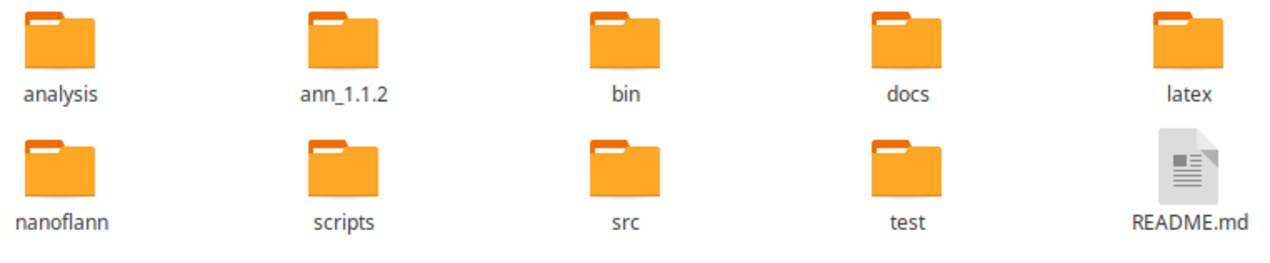
\includegraphics[width=0.75\textwidth]{figures/project_folders.pdf}
	\caption{The root-level structure of the project repository.}
      \label{FIG:folders}
\end{figure}

\section{Search Methods}
\label{SECTION:SRC}

The nearest neighbor search methods are implemented in C++. The \texttt{src} directory contains the source files. The linked-cell method is implemented in \texttt{fr\_cellLinkedList.cpp}. For the ANN method, there are multiple variants. First, \texttt{fr\_ann\_query.cpp} will only query a single query point for its neighbors. For the full nearest-neighbor search, a method that builds the interaction pair lists (\texttt{fr\_ann.cpp}) and a method that skips this step (\texttt{fr\_ann\_nolist.cpp}) are provided. This is necessary due to the extremely long time required for generating the interaction pair lists.

The \texttt{src} directory also contains a Makefile which can be used to build any or all of the source files. The resulting executable files are placed in the \texttt{bin} directory upon a successful build. Finally, source files for the Nanoflann library are provided (\texttt{fr\_nanoflann.cpp} and \texttt{utils.h}) for possible future work evaluating this additional  nearest neighbor search method.

\section{Test Case Scripts}
\label{SECTION:TESTCASESCRIPTS}

To be able to evaluate the performance of the different nearest neighbor search algorithms, a number of different test cases are required. These take the form of a list of data points which are processed by the search method run from the respective executables. The test cases differ by the distribution of the data points in the search domain and are described in detail in Section \ref{SECTION:TESTCASES}.

To generate the test cases, different scripts are used. Python was chosen as the scripting language due to familiarity and the availability of easy-to-use plotting libraries for visualization of the data point distributions. In the \texttt{scripts} directory, test case scripts are provided for four different distribution types examined in this work. With the exception of \texttt{test3d\_full}, which simply generates a filled domain, each of the scripts take certain parameters which control the fill and spacing of the points.  Note that due to the method used to generate the distributions, the fill factor passed to the script does not specify the fill directly - some experimentation is necessary to get the desired fill. 

The test case scripts are meant to be run within the benchmarking framework, as they also generate a statistics file for later use in the analysis. However, the scripts can also be run separately. Copy the script and the file \texttt{config.py} anywhere and execute the test case script with the Python interpreter. The data points are written to \texttt{data.pts} and can be visualized in 2D or 3D with scripts \texttt{plot\_2d.py} and \texttt{plot\_3d.py}.

\section{Jupyter Notebooks for Analysis}
\label{SECTION:NOTEBOOKS}

The Jupyter Notebooks found in the \texttt{analysis} directory are used to examine and compare the test results. To access the notebooks, make sure to have the appropriate packages installed (see Section \ref{SECTION:REQS}). The Jupyter Notebook server can be started from the project root with the command \texttt{jupyter notebook} and notebooks are viewed and executed via a web browser.

The notebook files themselves are generally self explanatory. The overall structure of the analysis is as follows. In the data-preparation notebook, data is read from the results files in the \texttt{tests} directory, cleaned and labeled, and then written to a CSV file. The following notebooks read the nicely-formatted data from the CSV file and generate various tables and plots. In other words, if the data in the \texttt{tests} directory changes, the data-preparation notebook must be rerun in order to update the CSV file.


\chapter{Test Cases \& Benchmarking Methodology}
\label{CHAPTER:BENCHMARKING}

This chapter first describes the test cases and shows how the data points are distributed for each case. Then, the benchmarking process and the tracked values are explained.

\section{Test Cases}
\label{SECTION:TESTCASES}

In SPH simulations of complex two-phase flows, particles can be distributed within the domain in a variety of different ways. They can be arranged in many small clusters, or large groups. The cluster edges can be arbitrarily oriented (aligned or unaligned with the coordinate system of the domain). Depending on the contents of the simulation domain, there can be many points in the domain or only relatively few. The test cases are designed to cover these different varieties and allow for a comparison between them.

The test cases are differentiated by two important parameters, {\itshape fill} and {\itshape fill type}. The distribution and orientation of the points is determined by the fill type. Specifically, there are four different fill types: \texttt{full}, \texttt{clusters}, \texttt{corners}, and \texttt{diagonal}. Each are generated using the appropriate test case script as described in Section \ref{SECTION:TESTCASESCRIPTS}.

The second important parameter is the fill. This is defined as the fraction of actual points in the domain over the number of points in a fully-filled domain. The test case \texttt{full}, consisting of a fully-filled domain, has by definition a fill of $1.0$. For a domain size of $0.005$x$0.01$x$0.005$ and a particle spacing of $10^{-4}$, the \texttt{full} test case contains 250000 points distributed on a regular grid. The number of points in the other test cases is therefore always a fraction of 250000. 

\begin{figure}[h]
	\centering
	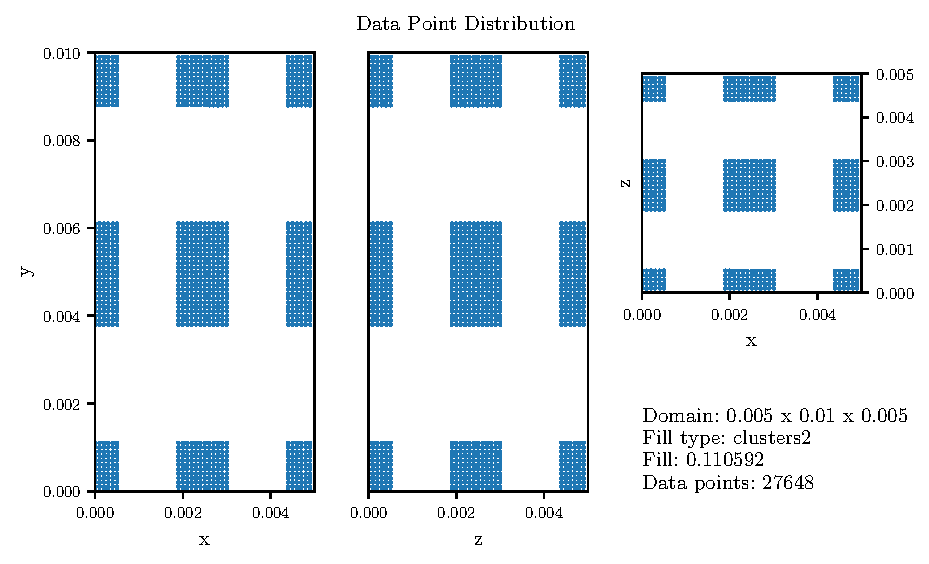
\includegraphics[]{figures/testcase_clusters2_11.pdf}
	\caption{Data points distribution for the clusters2 test case with 11\% fill.}
	\label{FIG:clusters2_11}
\end{figure}

The \texttt{clusters} test case is made up of rectangular, box-shaped clusters of points. Within the clusters, the points are distributed on a regular grid. The \texttt{clusters} cases are denoted \texttt{clustersN}, where the cluster size parameter $N$ specifies the number of clusters distributed throughout the space, i.e. a higher value of $N$ leads to more, but smaller clusters. The \texttt{clusters} test cases are examined for fill levels of 11\% and 51\% with varying cluster sizes. The cluster number parameter $N$ is set as an argument to the test case generation script. Exemplary \texttt{clusters} test cases for the same fill but different $N$ values can be see in Figure \ref{FIG:clusters2_11} and Figure \ref{FIG:clusters6_11}. 

\begin{figure}[h]
	\centering
	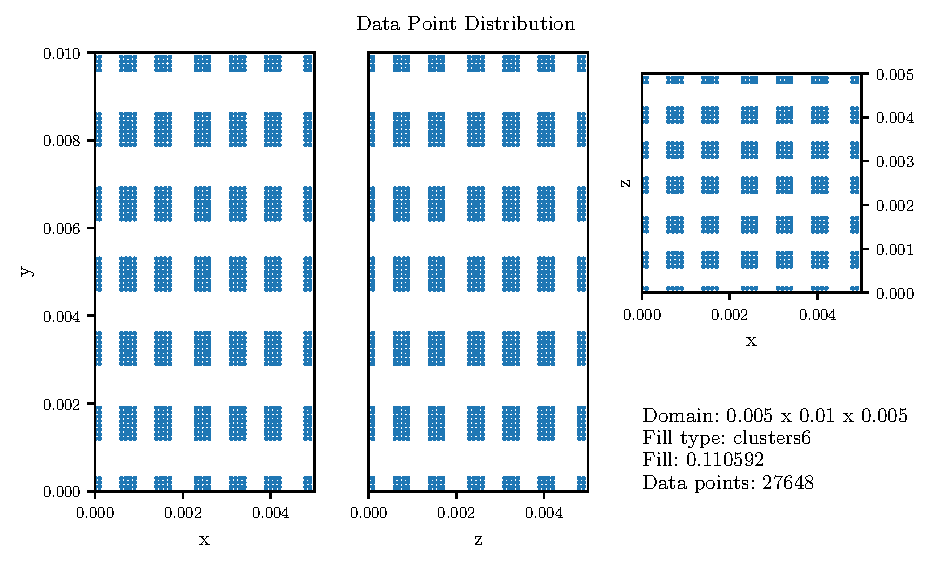
\includegraphics[]{figures/testcase_clusters6_11.pdf}
	\caption{Data points distribution for the clusters6 test case with 11\% fill.}
	\label{FIG:clusters6_11}
\end{figure}

The \texttt{corners} test case represent large groups of particles. The points are distributed regularly within two rectangular boxes extending from opposite corners of the domain towards the point in the center. This is visualized in Figure \ref{FIG:corners_11}. The maximum possible fill with this fill type is achieved when both boxes extend from their corners to the center. In this case two quarters of the domain are filled, leading to a fill of 50\%. The \texttt{corners} test case is examined for 2\%, 11\%, and 14\% fill.

\begin{figure}[h]
	\centering
	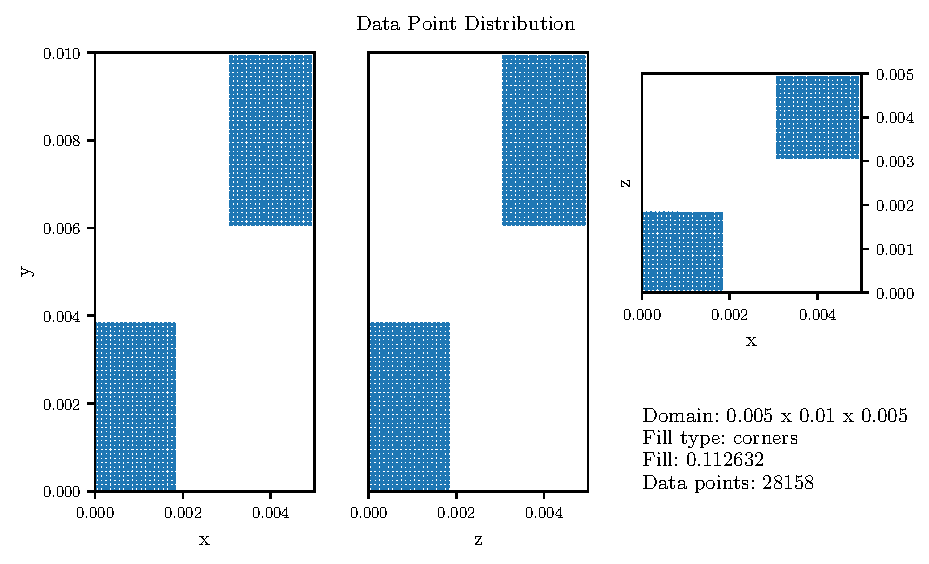
\includegraphics[]{figures/testcase_corners_11.pdf}
	\caption{Data points distribution for the corners test case with 11\% fill.}
	\label{FIG:corners_11}
\end{figure}

The \texttt{diagonals} test case is the only case in which the boundaries of the clusters are not parallel to the boundaries of the domain. The distribution is created by filling in the test domain from all eight corners up to a plane angled at 45 degrees from the domain boundaries. See Figure \ref{FIG:diagonals_11} for a 2D view of the \texttt{diagonals} test case with 11\% fill. This distribution is however best viewed in 3D using the \texttt{plot\_3d} script.

\begin{figure}[h]
	\centering
	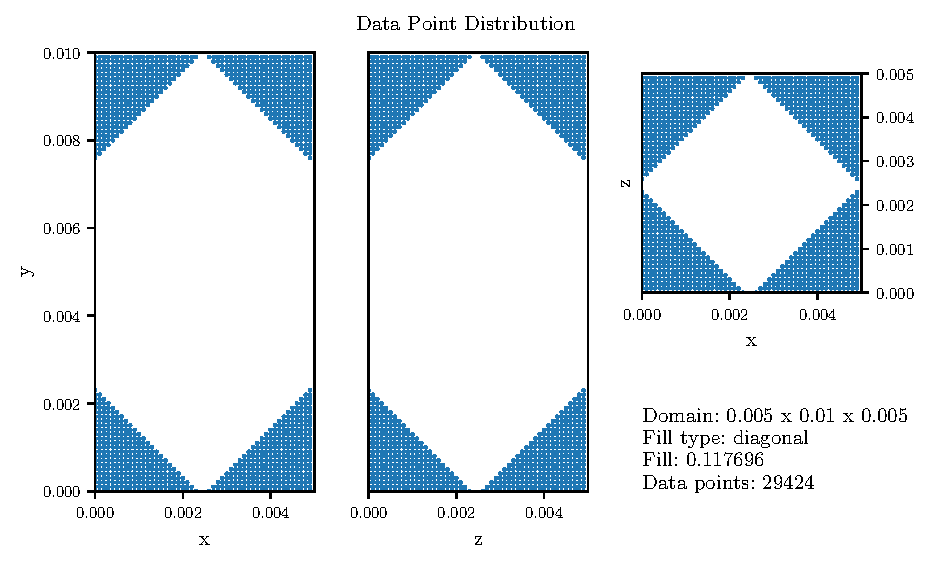
\includegraphics[]{figures/testcase_diagonal_11.pdf}
	\caption{Data points distribution for the diagonal test case.}
	\label{FIG:diagonals_11}
\end{figure}

\section{Table of Test Cases}

The following table (Table \ref{TABLE:TESTCASES}) contains an overview of which search methods were benchmarked for each test case. The cases marked with a dot were tested. The cases not marked were not tested due to excessively long runtimes.

\begin{table}[htbp]
	\centering
	\renewcommand{\arraystretch}{1.3} % Größerer Zeilenabstand
	\captionabove{Benchmarked test cases.}
	\begin{tabular}{lllll}
\toprule
     &     &        ANN &     ANN-NL &        CLL \\
filltype & fill &            &            &            \\
\midrule
clusters10 & 51  &            &  $\bullet$ &  $\bullet$ \\[2.0ex]
clusters2 & 11  &  $\bullet$ &  $\bullet$ &  $\bullet$ \\[2.0ex]
clusters20 & 51  &            &  $\bullet$ &  $\bullet$ \\[2.0ex]
clusters4 & 11  &  $\bullet$ &  $\bullet$ &  $\bullet$ \\[2.0ex]
clusters5 & 51  &            &  $\bullet$ &  $\bullet$ \\[2.0ex]
clusters6 & 11  &  $\bullet$ &  $\bullet$ &  $\bullet$ \\[2.0ex]
corners & 2   &  $\bullet$ &  $\bullet$ &  $\bullet$ \\
     & 11  &  $\bullet$ &  $\bullet$ &  $\bullet$ \\
     & 14  &            &  $\bullet$ &  $\bullet$ \\[2.0ex]
diagonal & 11  &  $\bullet$ &  $\bullet$ &  $\bullet$ \\
full & 100 &            &  $\bullet$ &  $\bullet$ \\
\bottomrule
\end{tabular}

	\label{TABLE:TESTCASES}
\end{table}


\section{Benchmarking}
\label{SECTION:BENCHMARKING}

This section describes the values that are tracked during benchmarking for the purpose of comparison of the search methods and how these values are collected with a scripted benchmarking process.

\subsection{Tracked values}

In order to compare the performance of the search methods, two characteristic values are tracked. The first is the run time of the search: how much time it takes for the program to solve the frNN search problem and compile the results into a useful data format. This is achieved by using timers within the C++ implementation of the search methods. For all search methods, the total time, \texttt{ttotal}, is tracked. This total time does not include reading or writing data. For the ANN search, the time is additionally split up into the time spent determining the number of neighbors, \texttt{tksearch}, the time spent retrieving the neighbors from the kd-tree structure, \texttt{tfrsearch}, and the time spent processing the interaction pair lists, \texttt{tprocessing}. The second tracked value is the memory use of the search method executable. This is measured by the \texttt{time} program, which outputs the maximum resident set size of the process. The resident set size is the space occupied by the process in the main memory (RAM).

\subsection{Benchmarking Process}

The benchmark is run via bash scripts for each search method, which define the test cases to run and also take care of tracking the memory use of the search processes. After the test case scripts and search method executables are copied to the test directory, the process as shown in Figure \ref{FIG:BENCHMARKING} is executed for each test case.

\begin{figure}[h]
	\centering
	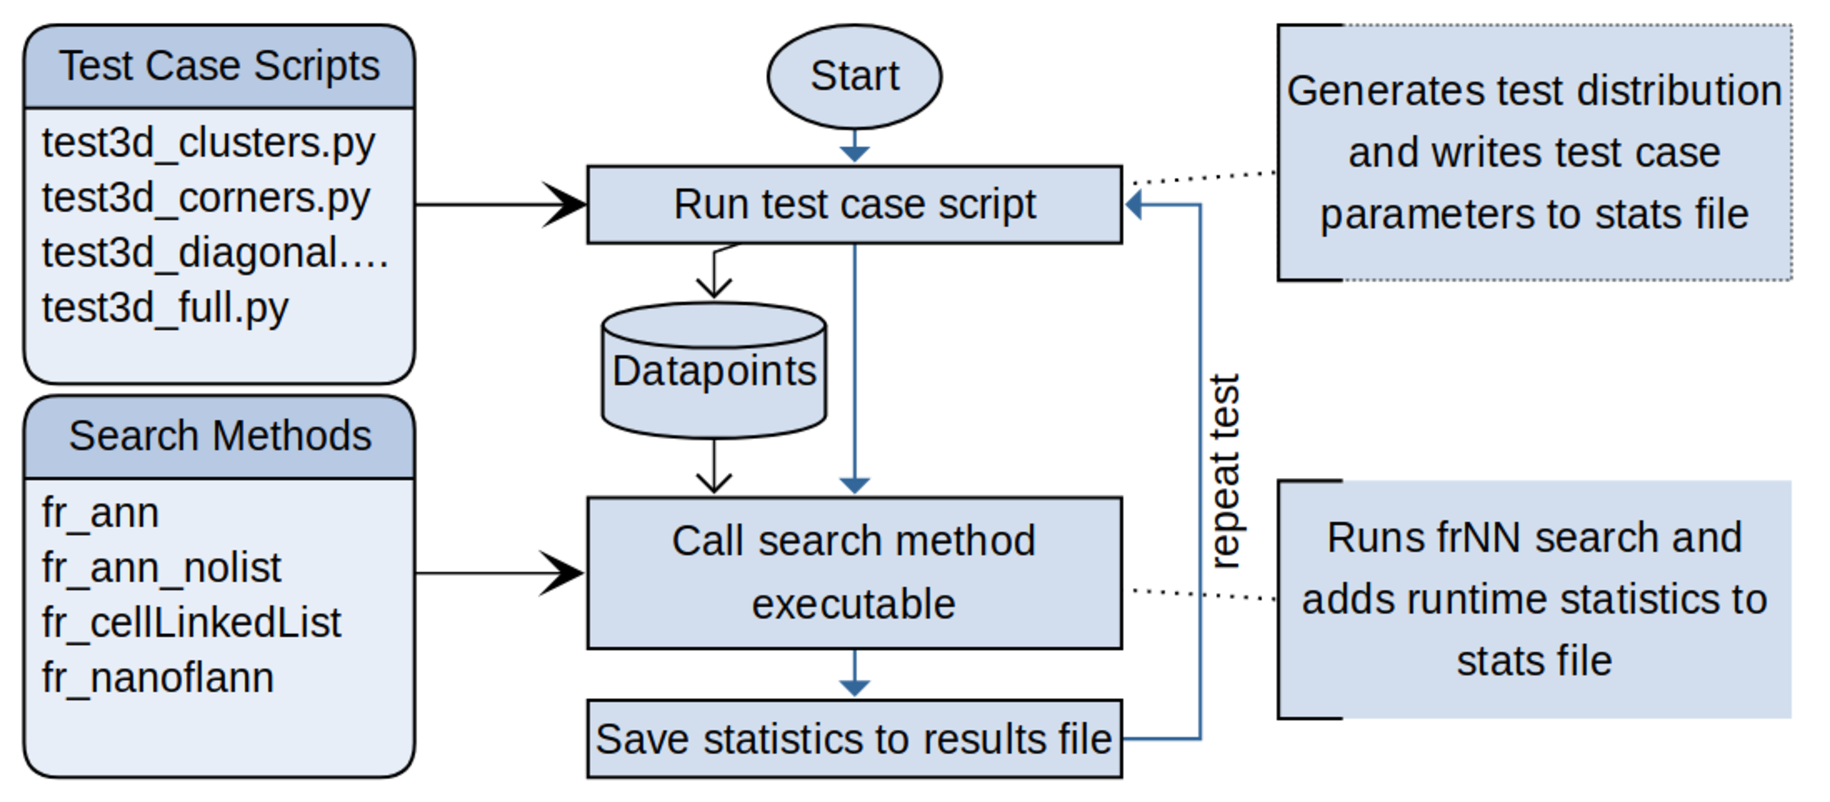
\includegraphics[width=0.75\textwidth]{figures/flowdiagram.pdf}
	\caption{The program flow for a test run with a certain test case and search method.}
	\label{FIG:BENCHMARKING}
\end{figure}

First, the test case script is called, which writes the data points and statistics file. The search method executable is then executed using the \texttt{time} command to track the memory use of the process. The search method executable adds its own time results to the statistics file and once it is finished the memory use results are also added. This is repeated multiple times to get a statistically valid sample. The script then moves on to the next test case, repeating the described process.




\chapter{Results and Discussion}

The results of the benchmarks were aggregated by mean over at least five repeated runs. The aggregated results can be found in Table \ref{TABLE:RESULTS} at the end of this chapter. Take special note of the extremely long runtimes for the ANN runs which include the interaction list processing. What follows is a graphical analysis of the benchmark results. First comes an overview of the results, followed by a more detailed breakdown of the search methods into the components and comparison over different fill types and fill percentages.

Figure \ref{FIG:runtimeall} shows the total runtime of the frNN search over various fill types. Each color represents a different a search method. The cell linked-list method ({\itshape CLL}) is in blue, the ANN library with interaction list processing in green, and the ANN library but without list processing (ANN-NoList, or {\itshape ANN-NL}) in orange. Note that there are no results for ANN for some test cases as the processing times for these cases exceeded reasonable values. The scattering in the x-axis does not have a meaning and is only to prevent overlapping of data points.

\begin{figure}[h]
	\centering
	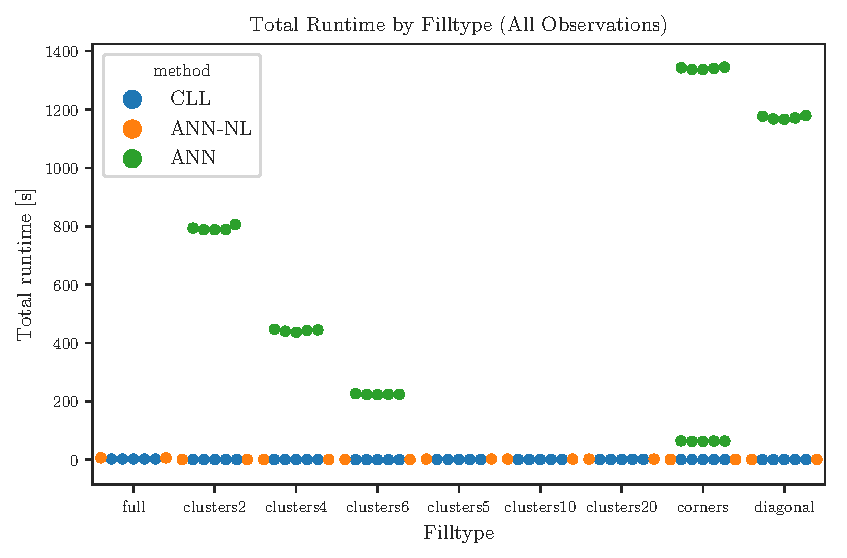
\includegraphics[width=\textwidth]{figures/totalruntime_all.pdf}
	\caption{Mean total runtime grouped by fill type.}
	\label{FIG:runtimeall}
\end{figure}

It is immediately apparent that the ANN runs take much longer than the other methods. In Figure \ref{FIG:runtimenoann}, ANN has been removed from the plot and only the CLL and ANN-NL runs are shown. With a more reasonable y-axis scale, we see that runtimes for ANN-NL are still significantly longer than CLL runtimes in almost all cases. In other words, the CLL method is faster and outputs the results in the correct format, while the ANN search itself takes longer and does not include the processing step.

\begin{figure}[h]
	\centering
	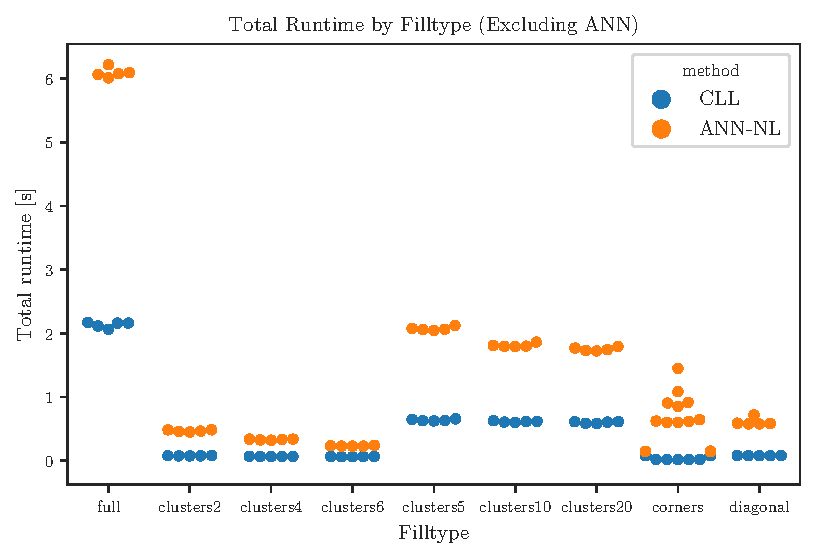
\includegraphics[width=\textwidth]{figures/totalruntime_noann.pdf}
	\caption{Total process runtime grouped by fill type, excluding ANN}
	\label{FIG:runtimenoann}
\end{figure}

\begin{figure}[h]
	\centering
	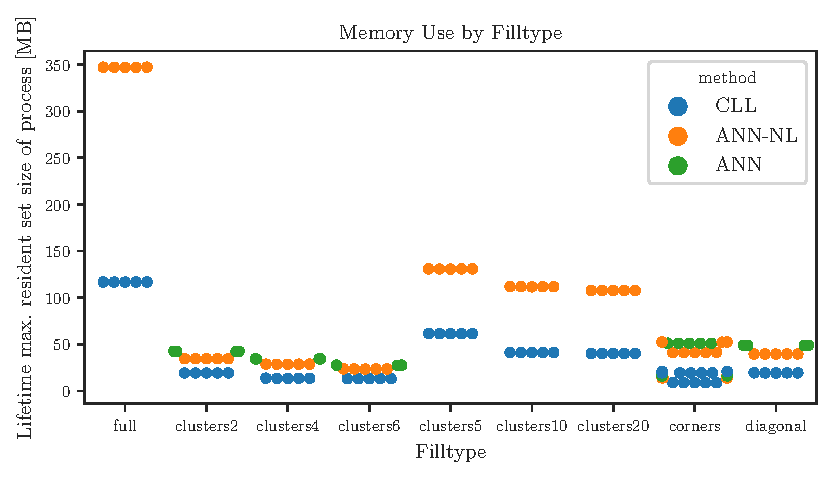
\includegraphics[width=\textwidth]{figures/memory_all.pdf}
	\caption{Mean maximum memory use grouped by filltype.}
	\label{FIG:memoryall}
\end{figure}

\pagebreak{}

Comparing memory use in Figure \ref{FIG:memoryall}, the ANN and ANN-NL methods are similar, with ANN-NL slightly below ANN. This is not surprising, as the memory requirements for the list generation are small compared to the kd-tree structure. However, the CLL method uses about one-half of the amount of memory that the ANN methods use.

Figure \ref{FIG:splitruntimeann} makes the expense of the list generation very clear by splitting the total runtime of the ANN search method into the search time and the list processing time. The runtimes are grouped by fill type and are averaged over different fills. The search time is made up of the time to find the number of neighbors of each point ({\itshape tksearch}, blue) and the time to retrieve the neighbors from the data structure ({\itshape tfrsearch}, yellow). The list processing time ({\itshape tprocessing}) is shown in a separate chart.  Note the different scales of the y-axes. 

\begin{figure}[h]
	\centering
	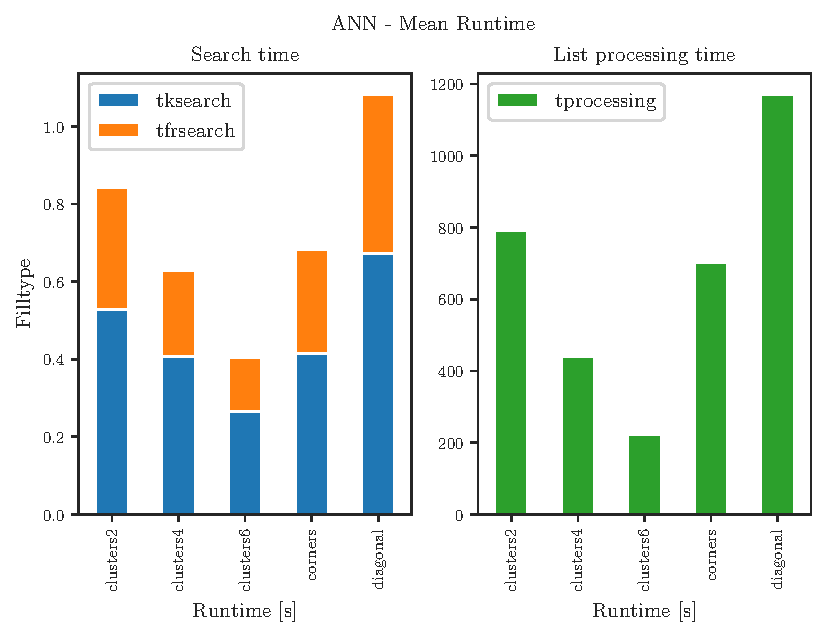
\includegraphics[width=\textwidth]{figures/ann_splitruntime.pdf}
	\caption{Total process runtime of the ANN search method split into search time (left) and interaction list processing time (right).}
	\label{FIG:splitruntimeann}
\end{figure}

The search times lie in a range of about 0.4 to 1.2 seconds. About $\frac{2}{3}$ of the search time is spend determining the neighbors and $\frac{1}{3}$ of it is spent retrieving the neighbors. The list processing times range from 200 to 1200 seconds, i.e. generating the interaction pair lists is 100x more expensive than the search itself. Therefore, for the ANN search method to be at all reasonable, either a significant performance increase in the list processing or a different approach that does not require the interaction lists at all must be found. 

\section{Effect of Fill}
\label{SECTION:ANALYSISFILL}

The fill was expected to have a significant effect on the runtime and memory use. Figure \ref{FIG:runtimefilltypes} shows, for each search type, the runtimes sorted from left to right by increasing fill percentage. For the ANN and ANN-NL methods, the total time is split into the neighbor search, neighbor retrieval, and list processing times. Some bars are very small due to the y-axis scale. See Table \ref{TABLE:RESULTS} for the actual values. The runtimes for the test cases with 11\% fill are also discussed in more detail in the next section. 

For the ANN search type, some results are not available as these benchmarks did not complete in reasonable time. Furthermore, the search and retrieval times are so small compared to the list processing time that they are not visible in the bar chart. Here it is only apparent that the fill percentage has the largest overall effect on the runtime. Going from 2\% to 11\% fill leads in the best case to a 3.5-fold increase in the total runtime. In the worst case, the total runtime for 11\% fill is 21 times that of the case with 2\% fill. With 51\% fill, the runtime exceeds 8 hours. Although not as extreme as the fill, the fill type also clearly has a large effect. This is discussed in more detail in Section \ref{SECTION:ANALYSISFILLTYPE}.

For CLL and ANN-NL the total runtime also generally increases with increasing fill percentage. From 11\% to 51\% fill, the CLL method runtime increases about 7.8 times and the ANN-NL method increases 4.1 times. From 51\% to 100\% fill, the CLL method runtime increases about 3.5 times and the ANN-NL method increases 3.3 times. Therefore we could say that the CLL method is probably more sensitive to the fill percentage in sparsely filled domains ($< 50\%$ fill) than the ANN-NL search. However, in all cases examined here, the CLL method was still significantly faster than ANN-NL even at very low fills. For example, at 2\% fill, ANN-NL requires 0.15s while CLL requires only 0.02s and and already outputs the interaction pair lists as required by the current SPH implementation.

\begin{figure}[h]
	\centering
	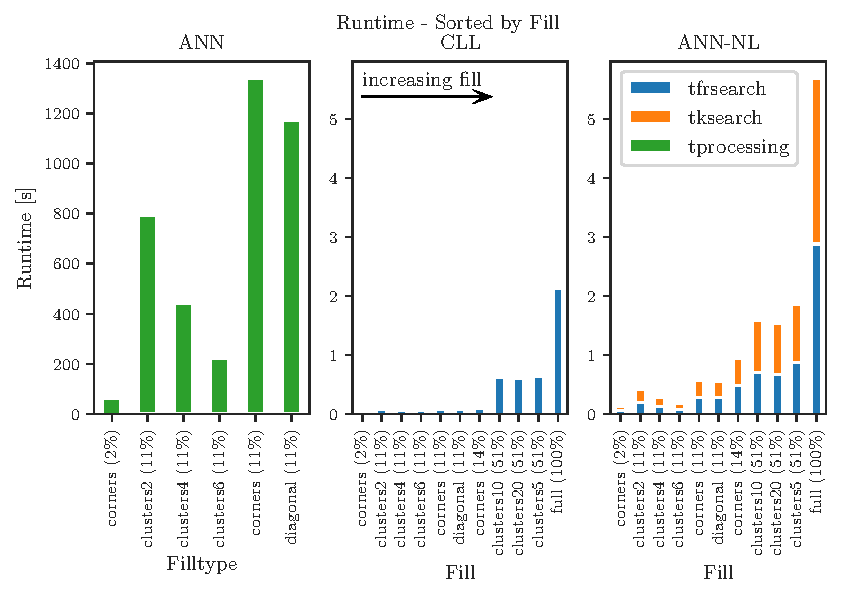
\includegraphics[width=\textwidth]{figures/runtime_filltypes.pdf}
	\caption{Total process runtimes sorted by fill percentage, for different search methods} 
	\label{FIG:runtimefilltypes}
\end{figure}

Figure \ref{FIG:memoryfilltypes} shows the maximum memory use of the search processes for each search type, with the fill again increasing from left to right. The memory use generally shows the same trends as the runtime results. Here as well CLL has an advantage over the ANN and ANN-NL search methods. The difference between ANN and ANN-NL is nowhere near as great as in the runtime. ANN-NL unsurprisingly requires less memory than ANN, as it does not have to store the interaction lists. But its clear that the bottleneck in the list generation step for high fills is in processing power and not memory.

\begin{figure}[h]
	\centering
	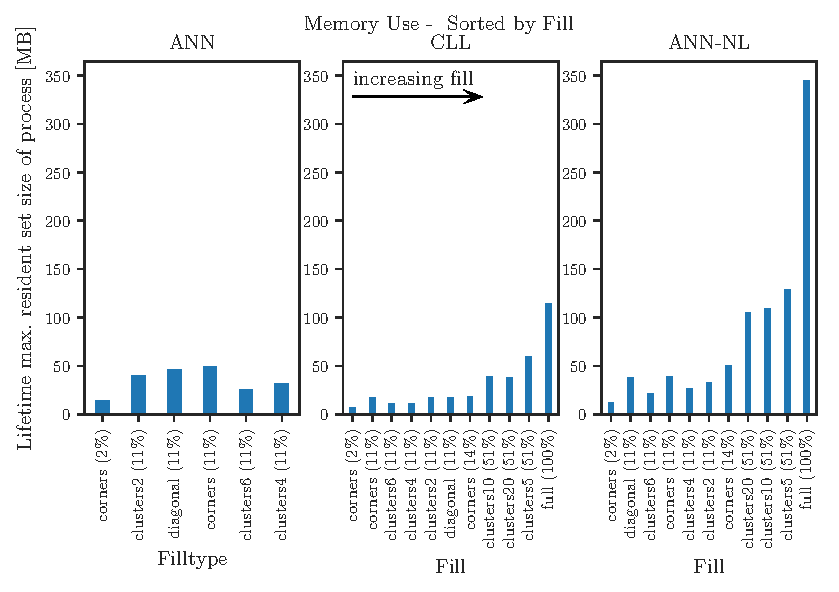
\includegraphics[width=\textwidth]{figures/memory_filltypes.pdf}
	\caption{Maximum memory use sorted by fill percentage, for different search methods} 
	\label{FIG:memoryfilltypes}
\end{figure}

\section{Effect of Fill Type}
\label{SECTION:ANALYSISFILLTYPE}

This section discusses the effect of effect of various particle distributions. For example, there could be only a few larger clusters in the domain, or many small clusters. The effect of vertical/horizontal or angled cluster boundaries is also examined briefly. In the following, various fill types are compared for the same amount of particles in the domain. The test cases following in this section are made up of between 27648 and 29424 points in the domain, which equates to between 11.06 and 11.70 percent fill.

Figure \ref{FIG:runtimefill11} shows the total runtime for each filltype for each search method. Only the results with a fill of 11\% are shown, and the total time is split into neighbor search, neighbor retrieval, and list processing time for ANN and ANN-NL search methods. The runtime on the y-axis of the figure is cut off at 1.5 seconds to facilitate comparison between the search methods. To see total runtimes for the ANN method refer back to Figure \ref{FIG:runtimefilltypes}.

A note on the cluster sizes for the 5 fill types shown here: The {\itshape corners} fill type has the largest clusters of all fill types, as all points are arrayed in two clusters in opposite corners of the domain. The {\itshape diagonals} follows close behind, with the particles distributed in 8 clusters. Then, for the {\itshape clusters} cases, the {\itshape clusters2} fill type has the largest clusters, {\itshape clusters4} is in-between, and {\itshape clusters6} has the smallest clusters. Refer also to the figures in Section \ref{SECTION:TESTCASES}.

\begin{figure}[h]
	\centering
	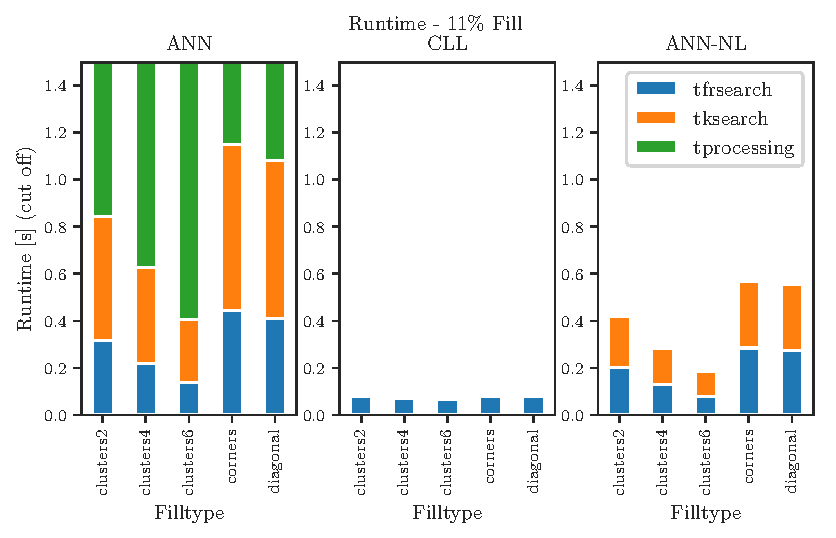
\includegraphics[width=\textwidth]{figures/runtime_fill11.pdf}
	\caption{Total process runtimes for various fill types at 11\% fill.}
	\label{FIG:runtimefill11}
\end{figure}

The total runtime of the CLL method is not significantly affected by the fill type. The results for the ANN methods do show an effect. It can be seen in the {\itshape clusters} cases that smaller clusters generally lead to a decrease in the runtime.

There is no significant difference between the {\itshape diagonal} and {\itshape corners} fill types. However, it was expected that the diagonal case would faster than the corners case, based on the difference in cluster sizes. So there could in fact be a negative impact on performance when the cluster boundaries are not orthogonal or parallel to the domain bounds. However, proving this definitively requires more test cases.

Interestingly, when ignoring the list processing time, ANN-NL method is significantly faster than the ANN method. This was not expected, as the only difference between the ANN and ANN-NL methods is the commenting-out of the source code for the list processing. Without closer examination, this is chalked up to some compiler optimizations or similar effects.

In Figure \ref{FIG:memoryfill11} the memory use of the search methods for each fill type for a fill of 11\% are shown. The trend again is aligned closely with the results for the runtime, with smaller clusters reducing the memory required and little difference between the {\itshape diagonal} and {\itshape corners} fill types. ANN-NL requires a bit less memory than ANN, as expected. For the CLL search method, there is a small difference visible in the memory use for the smallest clusters ({\itshape clusters4} and {\itshape clusters6}). 

\begin{figure}[h]
	\centering
	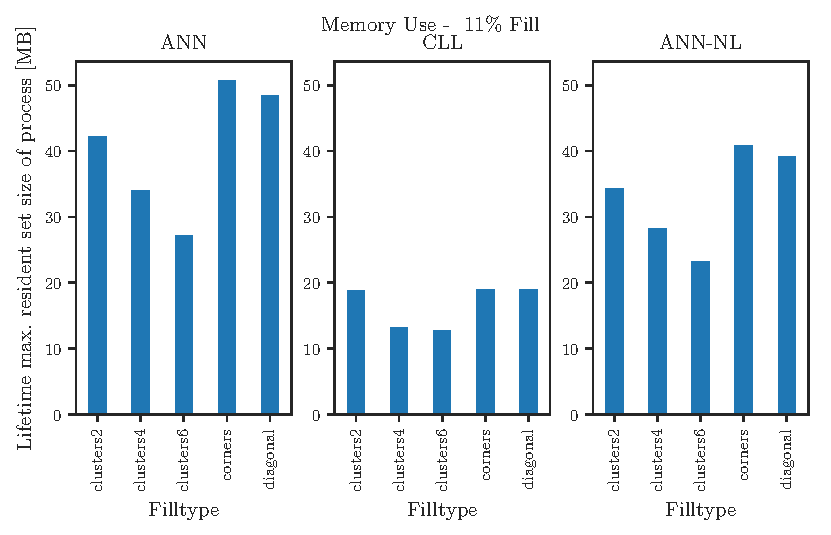
\includegraphics[width=\textwidth]{figures/memory_fill11.pdf}
	\caption{Maximum memory use for various fill types at 11\% fill.}
	\label{FIG:memoryfill11}
\end{figure}

\begin{table}[htbp]
	\centering
	\renewcommand{\arraystretch}{1.3} % Größerer Zeilenabstand
	\captionabove{All benchmarking results aggregated by mean.}
	\begin{tabular}{lllrrrrrr}
\toprule
    &      &     &  Datapts &  Memory &  $t_{frsearch}$ &  $t_{tksearch}$ &  $t_{processing}$ &  $t_{total}$ \\
fill & filltype & method &          &         &                 &                 &                   &              \\
\midrule
2 & corners & ANN &     7200 &   16.02 &            0.09 &            0.13 &             63.17 &        63.40 \\
    &      & ANN-NL &     7200 &   13.93 &            0.07 &            0.07 &              0.00 &         0.15 \\
    &      & CLL &     7200 &    8.84 &            0.00 &            0.00 &              0.00 &         0.02 \\[2.0ex]
11 & clusters2 & ANN &    27648 &   42.46 &            0.32 &            0.53 &            791.79 &       792.70 \\
    &      & ANN-NL &    27648 &   34.55 &            0.20 &            0.22 &              0.00 &         0.47 \\
    &      & CLL &    27648 &   19.18 &            0.00 &            0.00 &              0.00 &         0.08 \\
    & clusters4 & ANN &    27648 &   34.30 &            0.22 &            0.41 &            441.36 &       442.04 \\
    &      & ANN-NL &    27648 &   28.62 &            0.13 &            0.15 &              0.00 &         0.33 \\
    &      & CLL &    27648 &   13.50 &            0.00 &            0.00 &              0.00 &         0.07 \\
    & clusters6 & ANN &    27648 &   27.53 &            0.14 &            0.26 &            223.46 &       223.92 \\
    &      & ANN-NL &    27648 &   23.46 &            0.08 &            0.11 &              0.00 &         0.23 \\
    &      & CLL &    27648 &   13.03 &            0.00 &            0.00 &              0.00 &         0.07 \\
    & corners & ANN &    28158 &   51.01 &            0.45 &            0.70 &           1339.18 &      1340.39 \\
    &      & ANN-NL &    28158 &   41.14 &            0.28 &            0.28 &              0.00 &         0.62 \\
    &      & CLL &    28158 &   19.25 &            0.00 &            0.00 &              0.00 &         0.08 \\
    & diagonal & ANN &    29424 &   48.75 &            0.41 &            0.67 &           1170.92 &      1172.07 \\
    &      & ANN-NL &    29424 &   39.53 &            0.28 &            0.28 &              0.00 &         0.61 \\
    &      & CLL &    29424 &   19.27 &            0.00 &            0.00 &              0.00 &         0.08 \\[2.0ex]
14 & corners & ANN-NL &    37044 &   52.37 &            0.48 &            0.47 &              0.00 &         1.04 \\
    &      & CLL &    37044 &   20.88 &            0.00 &            0.00 &              0.00 &         0.10 \\[2.0ex]
51 & clusters10 & ANN-NL &   128000 &  111.68 &            0.71 &            0.89 &              0.00 &         1.81 \\
    &      & CLL &   128000 &   41.08 &            0.00 &            0.00 &              0.00 &         0.62 \\
    & clusters20 & ANN-NL &   128000 &  107.62 &            0.67 &            0.87 &              0.00 &         1.75 \\
    &      & CLL &   128000 &   40.04 &            0.00 &            0.00 &              0.00 &         0.60 \\
    & clusters5 & ANN-NL &   128000 &  130.79 &            0.87 &            0.99 &              0.00 &         2.07 \\
    &      & CLL &   128000 &   61.42 &            0.00 &            0.00 &              0.00 &         0.64 \\[2.0ex]
100 & full & ANN-NL &   250000 &  347.17 &            2.88 &            2.80 &              0.01 &         6.09 \\
    &      & CLL &   250000 &  116.75 &            0.00 &            0.00 &              0.00 &         2.14 \\
\bottomrule
\end{tabular}

	\label{TABLE:RESULTS}
\end{table}

\chapter{Summary and Outlook}


Increasingly stringent efficiency and emissions requirements for commercial turbofan engines have spurred the development of geared engine designs. To master the challenge presented by these engines in the form of gearbox cooling and lubrication, accurate and efficient simulation tools are currently being developed and improved. The smoothed-particle hydrodynamics method (SPH) is one such computational fluid dynamics tool that is used to evaluate the flow and distribution of oil in such a gearbox. The goal of this work was to examine an approach to increasing the computational efficiency of an SPH solver.

As a particle-based method, SPH requires an interaction-search step, where the solver determines which particles in the computational domain interact with each other. The approach in this work targets this interaction search step, which is mathematically a fixed-radius near-neighbor search. Currently, the solver uses the cell linked-lists method. It was expected that in sparsely-filled computational domains with few particles, other methods would have a performance advantage over the CLL method in the form of reduced run time or memory use.

To examine this hypothesis, a benchmarking framework was developed in which different search methods can be evaluated without running the full SPH code. The tracked values include the runtime of the search process or individual sections of the process, and the maximum memory use of the process. A modular approach was chosen in which the test cases, search methods, and results evaluation code can be replaced as required. 

The search methods are implemented in the same programming language as the SPH code, C++. They read in a list of particles representing a test case, and evaluate the neighbor search. The search methods include additional timing code to enable monitoring of the runtime. In addition to the CLL method, a C++ library called {\itshape ANN}, which implements a kd-tree data structure specifically for point neighbor searches, is evaluated. A third library, {\itshape nanoflann}, is mentioned but was not evaluated in detail due to time constraints.

Various test cases are generated using Python scripts. The test cases differ in two ways. First in the fill percentage, or how much of the domain contains particles. The second differentiating factor is the fill type, or how these points are distributed in the domain. For example, fewer but larger clusters of particles are expected to have different properties for neighbor searches then many clusters containing fewer particles. Clusters with boundaries that are not orthogonal or parallel to the edges of the domain are also tested.

After evaluating each of the test cases with the CLL and ANN search methods, it is immediately apparent that the ANN search method is much more computationally expensive than the CLL method in all test cases. This is due to the interaction pair list generation step, which must be completed separately when using ANN. Even with this step removed from the code (see ANN-NL results), the ANN method is significantly slower than the existing CLL method, which already includes the interaction list generation step. Futhermore, the CLL method uses about one-half of the amount of memory that the ANN method requires.

In addition to the comparison between the CLL and ANN methods. The effect of the parameters fill percentage and fill type were evaluated. Generally, processing time and memory use increases with the fill percentage due to the larger number of particles to be processed. The CLL method is not significantly influenced by the fill type. The ANN method is more sensitive and performs better (less memory and lower runtime) as the clusters get smaller. An influence of the cluster boundary orientation (orthogonal/parallel or diagonal) was seen, with diagonal boundaries leading to worse serach performance. However, due to the limited number of test cases this can not be definitively stated as fact without a more thorough examination.

Overall, the results show that the ANN search method approach does not yield any kind of performance improvement for the SPH simulation. The neighbor search itself is significantly slower than the CLL method. Even if the search itself were faster, the additionally required list processing step as implemented here is extremely  expensive computationally. In the current version of the SPH solver, which requires the interaction pair lists, the ANN method is not usable.

In future work, the Nanoflann library should be evaluated more closely. If the Nanoflann library is faster than the ANN library, and if the SPH code can be refactored to make better use of the kd-tree data structure, performance improvements for sparse domains are still conceivable.  Specifically, nanoflann theoretically supports updating parts of the search structure instead of rebuilding the entire structure. Alternative data storage methods such as bd-trees may also yield increased performance over kd-trees. For this and other alternative approaches, this work provides a good basis for further investigation.

%% Auf ungerader Seite starten
\cleardoublepage

%%%%%%%%%%%%%%%%%%%%%%%%%%%%%%%%%%%%%%%%%%%%%%%%%%%%%%%%%%%%%%%%%%%%%%%%%%%%%%%%%%%%%%%%%
% Einleitung
%%%%%%%%%%%%%%%%%%%%%%%%%%%%%%%%%%%%%%%%%%%%%%%%%%%%%%%%%%%%%%%%%%%%%%%%%%%%%%%%%%%%%%%%%

\chapter{Introduction}
\label{Chapter: Introduction}

Turbofan engines are widely used in commercial aircraft.  New, more stringent requirements with regards to emissions, fuel consumption and noise pollution are putting pressure on aircraft engine manufacturers to increase the efficiency of their products. From a technical point of view, there are two options: increase the thermal efficiency of the turbine stage or increase the bypass ratio of the engine. The bypass ratio is the amount of air that passes around the turbine core rather than through it.  Generally, a higher bypass ratio results in a quieter, more efficient engine. To increase the bypass ratio, the diameter of the engine's fan blades must be increased.  However, increasing the fan diameter leads to an increase in the circumferential velocity of the fan blade tips.  At very high speeds, large increases in losses and noise emissions are observed.

In conventional turbofans, the fan and the low-pressure compressor and turbine which drives the fan are attached to single shaft.  In this configuration, the speed of the compressor stage is limited by the blade tip speeds to the fan.  With the addition of a gearbox between the fan and the compressor and turbine, the fan speed can be greatly reduced while the compressor and turbine can rotate much faster.  Both components can therefore operate at their optimal speeds, greatly increasing efficiency and reducing noise.

However, geared turbofans are not without drawbacks.  In addition to increased complexity and manufacturing cost, a significant amount of energy is lost as heat within the gearbox.  The cooling and lubrication of the gearbox are key challenges.  These functions are realized with oil jets arranged around the gears.  The interaction between the oil jets and the gear surfaces determines the cooling and lubrication performance as well as the further propagation of the oil within the gearbox.

Therefore, this interaction is a current focus of research at the Insitute of Thermal Turbomachinery at the Karlsruhe Institute of Technology.  Experimental investigations in this area are difficult due to the small time scale and inaccessible location of the interactions. However, Computational Fluid Dynamics (CFD) methods offer possibilities for detailed investigation. One such method is Smoothed Particle Hydrodynamics (SPH), a particle-based method that is well-suited to modeling free surface flows and moving boundaries.  SPH, like other approaches to fluid dynamics modeling, is very computationally expensive.

It is desirable to reduce the required computation time as much as possible. For this purpose, this work examines an approach to increasing the computational efficiency of the SPH solver and therefore reducing the required computation time. 

\chapter{Objective}

\section{Motivation}
\label{SECTION:Motivation}
Smoothed-particle hydrodynamics is a computational method which can be used to simulate mechanics of solids and fluids.  It is mesh-free and employs the Lagrangian approach, which makes it well-suited for complex problems with free surface flows and moving boundaries.

Compared to mesh-based methods, SPH requires a very large number of particles to ensure an equivalent resolution.  However, in applications where there is relatively little high-density fluid (e.g.  oil) in a computational space filled with low-density fluid (e.g.  air), the low-density phase cam be completely omitted.  This is results in a sparse computational domain, in which the amount of particles is small compared to the size of the domain.

During an SPH-method simulation, particles interact locally within a characteristic radius ("smoothing length").  In other words, each particle's behavior is influenced only by the particles surrounding it within a certain range.  Therefore, for each particle $p_i$ in the domain, all points within a certain cut-off radius $r$ around the particle must be determined.  This type of search is called {\itshape fixed-radius near neighbor} (frNN) search.

In the in-house code currently in use at the Insitute for Thermal Turbomachinery, the fixed-radius near neighbors search is implemented using cell linked-lists (CLL, also cell lists). In sparsely-filled computational domains as seen in simulations using the SPH method, other methods for frNN search may yield a performance advantage over the CLL method, in the form of reduced run time or decreased memory use.

\section{Problem}
\label{SECTION:Problem}
The fixed-radius near-neighbor search in this case is specified as follows:

{\itshape
For each point $p_i$ within the computational domain, find all neighbors $p_j$ that lie less than a cut-off radius $r = 3d_x$ , away from the particle, where $d_x$ is the mean particle spacing. This includes the particle $p_1$itself. The result is a set of interactions $p_i \leftrightarrow p_j$, where  $p_j \leftrightarrow p_i $ is considered identical to $p_i \leftrightarrow p_j$ and is not repeated.}

\section{Objective}
\label{SECTION:Objective}
The objective of this work is to compare alternative methods for solving the described fixed-radius near neighbor search problem to the existing solution using CLL. For this purpose, a benchmarking framework is created in which the a comparison can take place independently of the rest of the SPH code. Alternative solutions are researched and the most promising methods are implemented within the framework along with the CLL method. The benchmarks measure process runtime and memory use, which are then used to compare the search methods.

\chapter{Neighbor Search Methods}

The following sections describe tools that can be used to solve the fixed-radius near neighbor search problem described in section~\ref{SECTION:Problem}. These are implemented in C++ 11 and outfitted with timing code in order to measure their execution times. 

\section{Cell Linked-Lists Method}

The cell-linked lists method (also called linked-cell method or cell-lists method) divides the calculation domain into cells of edge lengths equal to or greater than the cutoff radius of the interaction search. Therefore, to find the neighbors of a particle, only the cells adjacent to the cell containing the particle must be searched. In the 3D case, the potential neighbors of a particle are found within the 27 cells directly surrounding the particle (\cite{Weygand18}).

The particles themselves are first sorted into two lists, $first$ and $next$. The list $first$ contains the indices of the first particle in the cell for each cell, i.e.\ $first[i]$ is the first particle in the  $i$-th cell.   The list $next$ links a particle $i$ to the index of the next particle $j$ in the same cell, i.e. $next[i] = j$. If there are no further particles in the cell, $next$ contains $-1$. In this manner, by starting with the first particle and following the links until the next index is $-1$, all particles in a cell can be visited in an efficient manner.

To create particle interaction lists for the full domain, the search loops through each cell pair. A cell pair is the current cell and itself, or the current cell and an adjacent cell. For each particle in the current cell, the distance to each particle in the other cell is calculated. If the distance is smaller than the cutoff radius, the interaction is added to the interaction pair lists. For increased efficiency, there is no need to check ``backwards'' into previous adjacent cells, as any interactions between the current cell and the previous cell have already been found.

\section{The {\itshape ANN} Library}
\label{SECTION:ANN}


The ANN library, written by David M. Mount and Sinul Arya (\ref{ANN10}), implements k-nearest neighbor search using methods based on orthogonal space decomposition. The particles in the search domain are spatially sorted into special data structures. ANN supports kd-trees and box-decomposition trees (bd-tress). The bd-tree includes more decomposition methods than the kd-tree and is more robust for highly clustered data sets. 

ANN supports exact and approximate nearest neighbor searching and a number and a number of distance metrics. In this case, the ANN library is used to perform exact fixed-radius NN searching using the Euclidean ($L_2$) distance metric. Exact searches can be performed by setting the tolerance $\epsilon$ to 0. For fixed-radius searching, ANN provides a procedure $annkFRSearch$, which returns the $k$ closest points that lie within the radius bound. Because ANN statically allocates its arrays, the $annFRSearch$ function must be called twice to find all points within the radius: once to find the number of points within the radius, and a second time to actually find the points.

The procedure as implemented in this work is therefore as follows:  First, the search tree structure is initialized using the all data points (particles) in the search domain. Then the $annkFRSearch$ procedure is called twice for each data point. Initially, a search is performed using $annkFRSearch$ with $k = 0$ to find the number of points $k'$ that lie within the radius bound.  Then, the appropriate arrays of size $k'$ are allocated, and filled by calling the procedure a second time with $k = k'$. At this point, the neighbors and therefore the interactions of the current point are known. These must then be inserted into the interaction lists, making sure not to duplicate any interactions.

If there is a known upper bound on the possible number of points within the search radius, it would be possible to pre-allocate arrays that are as large as the upper bound, and therefore need to perform the search only once. It is assumed that this would come at the cost of higher memory use, but it was not tested in the scope of this work. For more detailed information about the ANN libraby, see the ANN Programming Manual (\ref{ANN10}).

\section{The {\itshape nanoflann} Library}
\label{SECTION:NanoFLANN}
{\itshape nanoflann} is a header-only library for C++11 for KD-Tree structures.  It does not support approximate nearest neighbors search.  It includes a number of optimizations for increased efficiency.  For instance, there are no provisions for choosing between or adding custom NN-search algorithms, and by using STL containers for the output data, there is no need to call the fixed-radius search method twice, as is the case with ANN. \ref{FIXME}.

These optimizations could lead to performance advantages of {\itshape nanoflann} over the {\itshape ANN} library. It is also able to work with dynamic point clouds without rebuilding the entire kd-tree index. For these reasons, it could be promising for the final application and is mentioned here and included in the source files. However, a comparison to the ANN library is not included in this report.


\chapter{Project Structure and Requirements}

This chapter describes the structure of the project. First the overall organization and then the individual components are explained. Following that, the prerequisites and processes for building and/or running the code used in various parts of the project are briefly described.

\section{Requirements}
\label{SECTION:REQS}
This project requires a Linux system with {\itshape gcc}, {\itshape bash}, and a recent version of Python 3 with the {\itshape numpy} package to run the benchmarks. Additional Python packages are required to view and execute the analysis notebooks. {\itshape Jupyter Notebook}, {\itshape matplotlib},  {\itshape pandas}, and {\itshape seaborne} can be installed using the python package installer {\itshape pip}. Note: Jupyter requires at least Python 3.3.

\section{Directory Structure}
Figure \ref{FIG:folders} shows the file structure of the project.  First of all, the documentation (i.e.  this pdf) is in the {\itshape docs} folder, and the latex source files are in {\itshape latex}. The {\itshape ann\_1.2.2} directory contains the neighbor search C++ libraries that is examined. The {\itshape nanoflann} directory is an additional neighbor search libraray (see section \ref{FIXME}.  The folders {\itshape src} and {\itshape bin} contain the C++ source files (described in section \ref{SECTION:SRC}) and their compiled binaries, respectively.  The {\itshape scripts} directory is home to the test case generation scripts (described in section \ref{SECTION:TESTS}) and test execution scripts (see chapter \ref{CHAPTER:BENCHMARKING}).  The {\itshape test} directory contains the working directories of the test runs and the result data.   Finally, the folder {\itshape analysis} contains the iPython notebooks that were used in the examination and analysis of the results.  These are described in more detail in section \ref{SECTION:NOTEBOOKS}.

\begin{figure}[h]
	\centering
	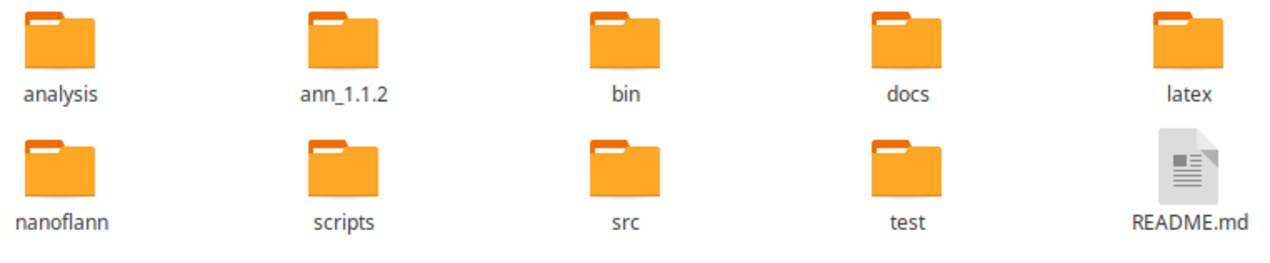
\includegraphics[width=0.75\textwidth]{figures/project_folders.pdf}
	\caption{The root-level structure of the project repository.}
      \label{FIG:folders}
\end{figure}

\section{Search Methods}
\label{SECTION:SRC}

The nearest neighbor search methods are implemented in C++ 11. The {\itshape src} directory contains the source files. The linked-cell method is implemented in {\itshape fr\_cellLinkedList.cpp}. For the ANN method, there are multiple variants. First, {\itshape fr\_ann\_query.cpp} will only query a query single point for its neighbors. For the full nearest neighbor search, a method that builds the interaction pair lists ({\itshape fr\_ann.cpp}) and a method that skips this step ({\itshape fr\_ann\_nolist.cpp}) are provided. This was necessary due to the extremely long time required for generating the interaction pair lists.

The {\itshape src} directory also contains a Makefile which can be used to build any or all of the source files. The resulting executable files are placed in the {\itshape bin} directory upon a successful build. Finally, source files for the Nanoflann library are provided ({\itshape fr\_nanoflann.cpp} and {\itshape utils.h}) for possible future work evaluating this additional  nearest neighbor search method. For more details about Nanoflann, see section \ref{SECTION:NanoFLANN}.

\section{Test Case Scripts}
\label{SECTION:TESTCASESCRIPTS}

To be able to evaluate the performance of the different nearest neighbor search algorithms, a number of different test cases are required. These take the form of a list of data points which are processed by the search method executable. The test cases differ by the distribution of the data points in the search domain and are described in detail in section \ref{FIXME}.

To generate the test cases, different scripts are used. Python was chosen as the scripting language due to familiarity and the availability of easy-to-use plotting libraries for visualization of the data point distributions. In the {\itshape scripts} directory, test case scripts are provided for four different distribution types examined in this work. With the exception of {\itshape test3d\_full}, which simply generates a filled domain, each of the scripts take certain parameters which control the fill and spacing of the points.

The test case scripts are meant to be run within the benchmarking framework, as they also generate a statistics file for later use in the analysis. However, the scripts can also be run separately. Copy the script and the file {\itshape config.py} anywhere and execute the test case script with the Python interpreter. The data points are written to {\itshape data.pts} and can be visualized in 2D or 3D with scripts {\itshape plot\_2d.py} and {\itshape plot\_3d.py}.



\section{Jupyter Notebooks for Analysis}
\label{SECTION:NOTEBOOKS}

To examine and compare the test results, Python is again used in the form of Jupyter Notebooks found in the {\itshape analysis} directory. To access the notebooks, make sure to have the appropriate packages installed (see \ref{SECTION:REQS}). The Jupyter Notebook server can be started from the project root and notebooks are viewed and executed via a web browser.

The notebook files themselves are generally self explanatory. The overall structure of the analysis is as follows. In the data-preparation notebook, data is read from the results files in the {\itshape tests} directory, cleaned and labeled, and then written to a CSV file. The following notebooks read the nicely-formatted data from the CSV file and generate various tables and plots. In other words, if the data in the {\itshape tests} directory changes, the data-preparation notebook must be rerun in order to update the CSV file.

\chapter{Test Cases \& Benchmarking Methodology}
\label{CHAPTER:BENCHMARKING}

\section{Running Tests}
\label{SECTION:TESTS}

\begin{figure}[h]
	\centering
	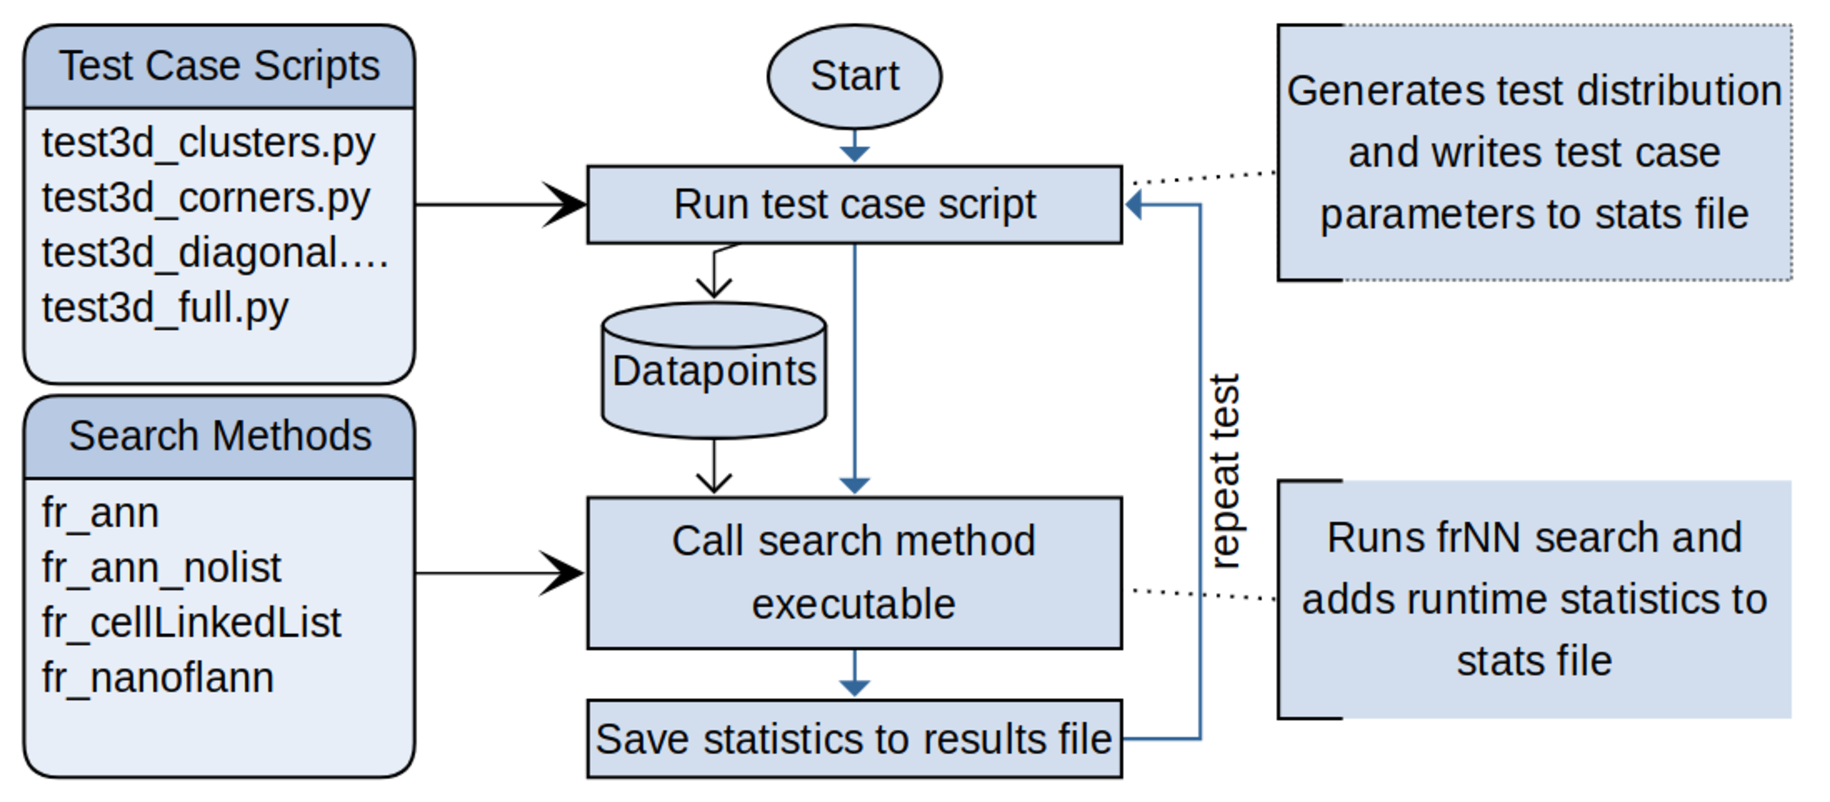
\includegraphics[width=0.75\textwidth]{figures/flowdiagram.pdf}
	\caption{The program flow for a test run with a certain test case and search method.}
\end{figure}


\section{Test Cases}

\section{Benchmarking}

Allows selection of list generation method. Initial tests comparing two list generation methods, it was clear that method1 (FIXME explain!) was about twice as fastas method0 (FIXME: explain). therefore the tests were completed with method 1. While method 0 gnerate 

\chapter{Results and Discussion}

\begin{table}[htbp]
	\centering
	\renewcommand{\arraystretch}{1.3} % Größerer Zeilenabstand
	\captionabove{Results (mean values)}
      \begin{tabular}{lllrrrrrr}
\toprule
    &      &     &  Datapts &  Memory &  $t_{frsearch}$ &  $t_{tksearch}$ &  $t_{processing}$ &  $t_{total}$ \\
fill & filltype & method &          &         &                 &                 &                   &              \\
\midrule
2 & corners & ANN &     7200 &   16.02 &            0.09 &            0.13 &             63.17 &        63.40 \\
    &      & ANN-NL &     7200 &   13.93 &            0.07 &            0.07 &              0.00 &         0.15 \\
    &      & CLL &     7200 &    8.84 &            0.00 &            0.00 &              0.00 &         0.02 \\[2.0ex]
11 & clusters2 & ANN &    27648 &   42.46 &            0.32 &            0.53 &            791.79 &       792.70 \\
    &      & ANN-NL &    27648 &   34.55 &            0.20 &            0.22 &              0.00 &         0.47 \\
    &      & CLL &    27648 &   19.18 &            0.00 &            0.00 &              0.00 &         0.08 \\
    & clusters4 & ANN &    27648 &   34.30 &            0.22 &            0.41 &            441.36 &       442.04 \\
    &      & ANN-NL &    27648 &   28.62 &            0.13 &            0.15 &              0.00 &         0.33 \\
    &      & CLL &    27648 &   13.50 &            0.00 &            0.00 &              0.00 &         0.07 \\
    & clusters6 & ANN &    27648 &   27.53 &            0.14 &            0.26 &            223.46 &       223.92 \\
    &      & ANN-NL &    27648 &   23.46 &            0.08 &            0.11 &              0.00 &         0.23 \\
    &      & CLL &    27648 &   13.03 &            0.00 &            0.00 &              0.00 &         0.07 \\
    & corners & ANN &    28158 &   51.01 &            0.45 &            0.70 &           1339.18 &      1340.39 \\
    &      & ANN-NL &    28158 &   41.14 &            0.28 &            0.28 &              0.00 &         0.62 \\
    &      & CLL &    28158 &   19.25 &            0.00 &            0.00 &              0.00 &         0.08 \\
    & diagonal & ANN &    29424 &   48.75 &            0.41 &            0.67 &           1170.92 &      1172.07 \\
    &      & ANN-NL &    29424 &   39.53 &            0.28 &            0.28 &              0.00 &         0.61 \\
    &      & CLL &    29424 &   19.27 &            0.00 &            0.00 &              0.00 &         0.08 \\[2.0ex]
14 & corners & ANN-NL &    37044 &   52.37 &            0.48 &            0.47 &              0.00 &         1.04 \\
    &      & CLL &    37044 &   20.88 &            0.00 &            0.00 &              0.00 &         0.10 \\[2.0ex]
51 & clusters10 & ANN-NL &   128000 &  111.68 &            0.71 &            0.89 &              0.00 &         1.81 \\
    &      & CLL &   128000 &   41.08 &            0.00 &            0.00 &              0.00 &         0.62 \\
    & clusters20 & ANN-NL &   128000 &  107.62 &            0.67 &            0.87 &              0.00 &         1.75 \\
    &      & CLL &   128000 &   40.04 &            0.00 &            0.00 &              0.00 &         0.60 \\
    & clusters5 & ANN-NL &   128000 &  130.79 &            0.87 &            0.99 &              0.00 &         2.07 \\
    &      & CLL &   128000 &   61.42 &            0.00 &            0.00 &              0.00 &         0.64 \\[2.0ex]
100 & full & ANN-NL &   250000 &  347.17 &            2.88 &            2.80 &              0.01 &         6.09 \\
    &      & CLL &   250000 &  116.75 &            0.00 &            0.00 &              0.00 &         2.14 \\
\bottomrule
\end{tabular}

\end{table}



\begin{figure}[h]
	\centering
	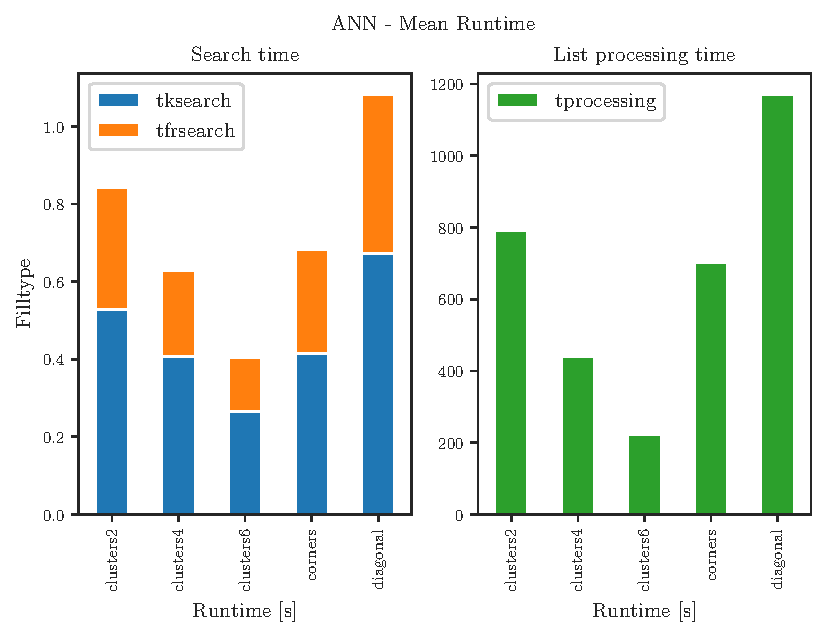
\includegraphics[width=\textwidth]{figures/ann_splitruntime.pdf}
	\caption{FIXME!}
\end{figure}

\begin{figure}[h]
	\centering
	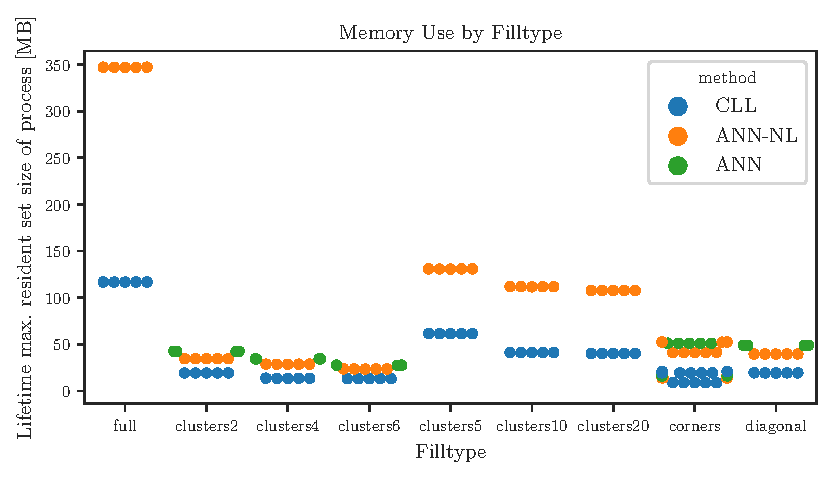
\includegraphics[width=\textwidth]{figures/memory_all.pdf}
	\caption{FIXME!}
\end{figure}
\begin{figure}[h]
	\centering
	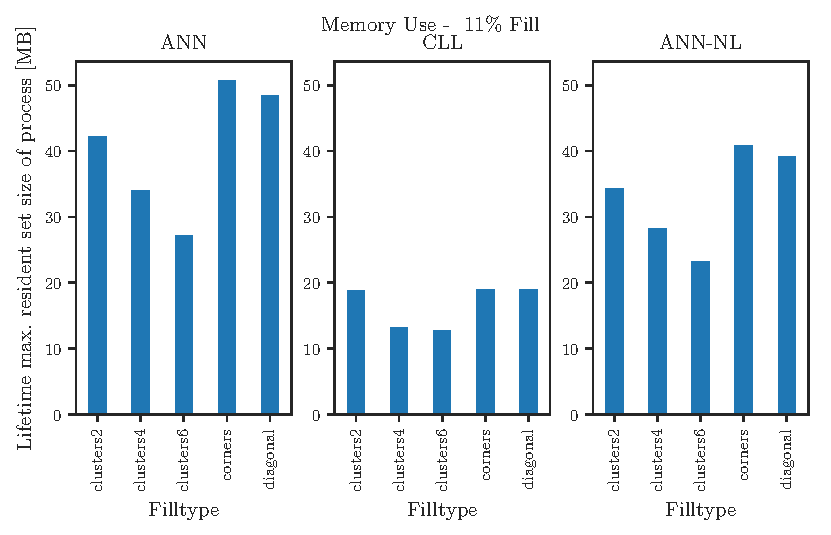
\includegraphics[width=\textwidth]{figures/memory_fill11.pdf}
	\caption{FIXME!}
\end{figure}
\begin{figure}[h]
	\centering
	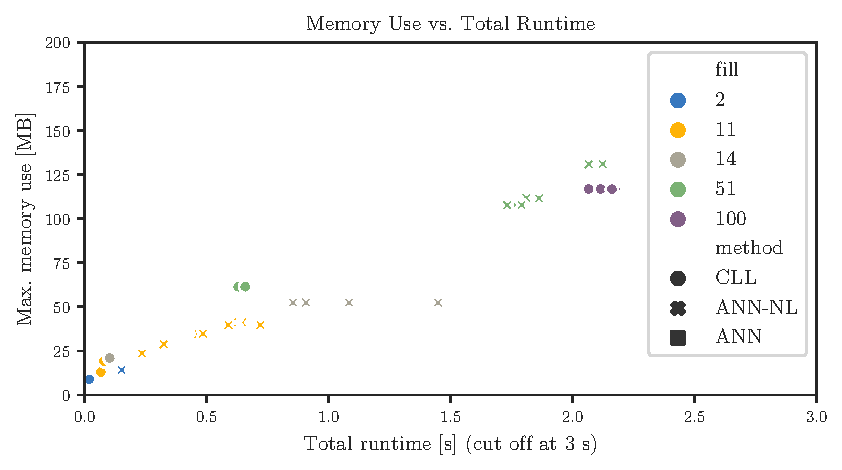
\includegraphics[width=\textwidth]{figures/memory_vs_totalruntime.pdf}
	\caption{FIXME!}
\end{figure}
\begin{figure}[h]
	\centering
	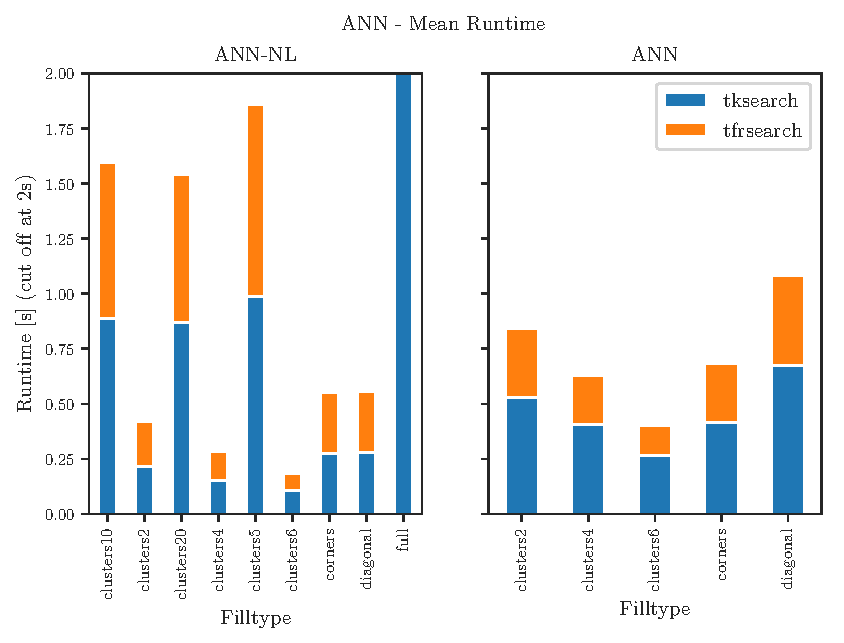
\includegraphics[width=\textwidth]{figures/runtime_ann_annnl.pdf}
	\caption{FIXME!}
\end{figure}
\begin{figure}[h]
	\centering
	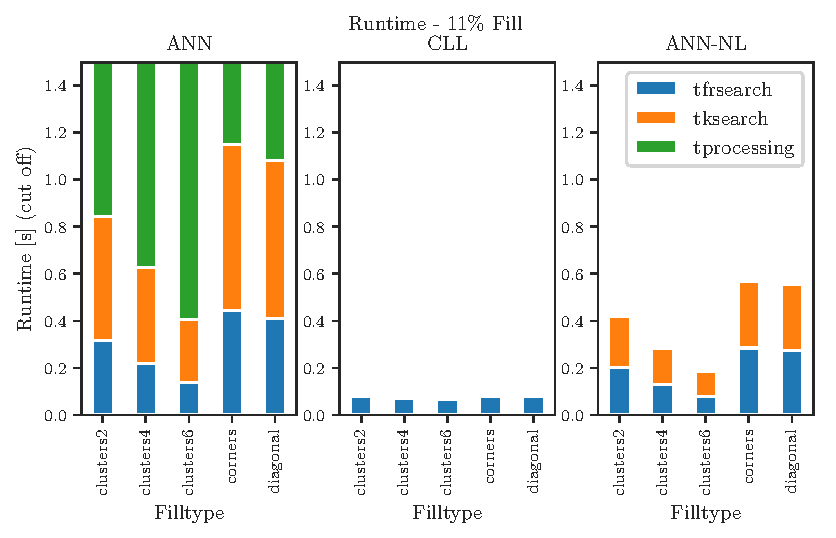
\includegraphics[width=\textwidth]{figures/runtime_fill11.pdf}
	\caption{FIXME!}
\end{figure}

\begin{figure}[h]
	\centering
	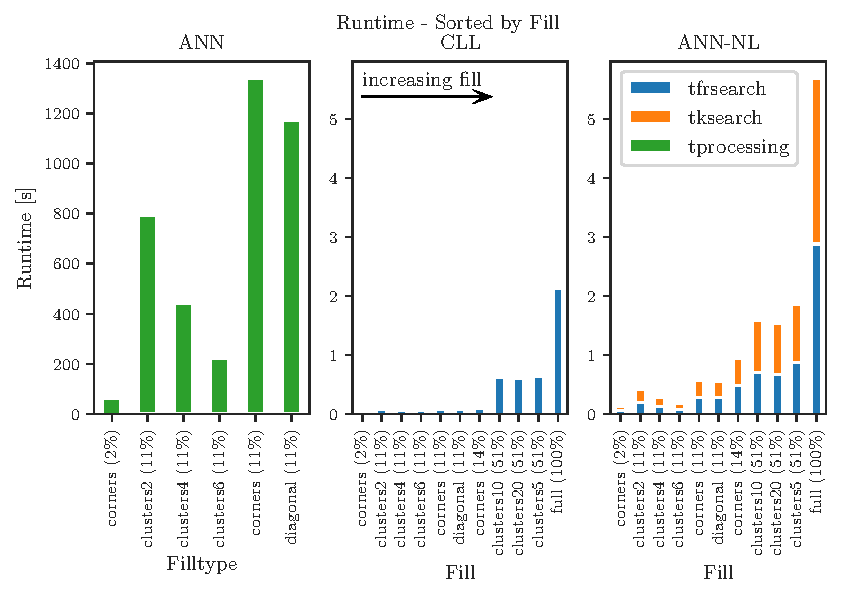
\includegraphics[width=\textwidth]{figures/runtime_filltypes.pdf}
	\caption{FIXME!}
\end{figure}

\begin{figure}[h]
	\centering
	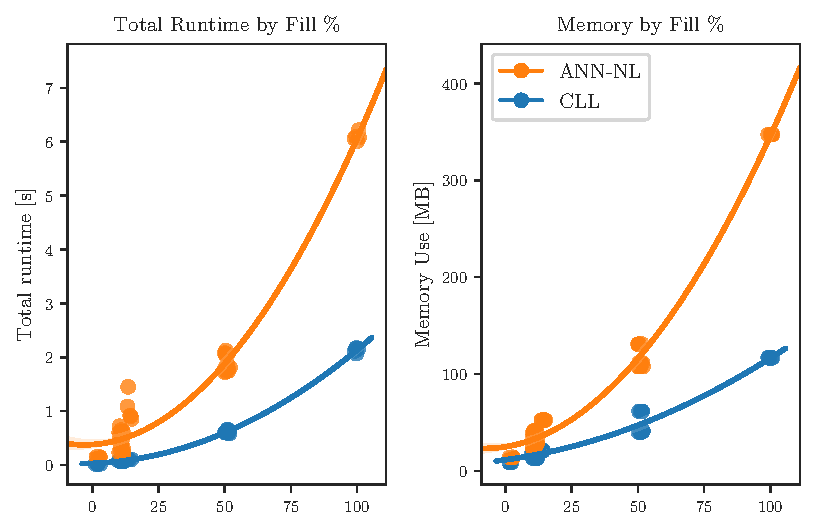
\includegraphics[width=\textwidth]{figures/runtime_vs_fill.pdf}
	\caption{FIXME!}
\end{figure}
\begin{figure}[h]
	\centering
	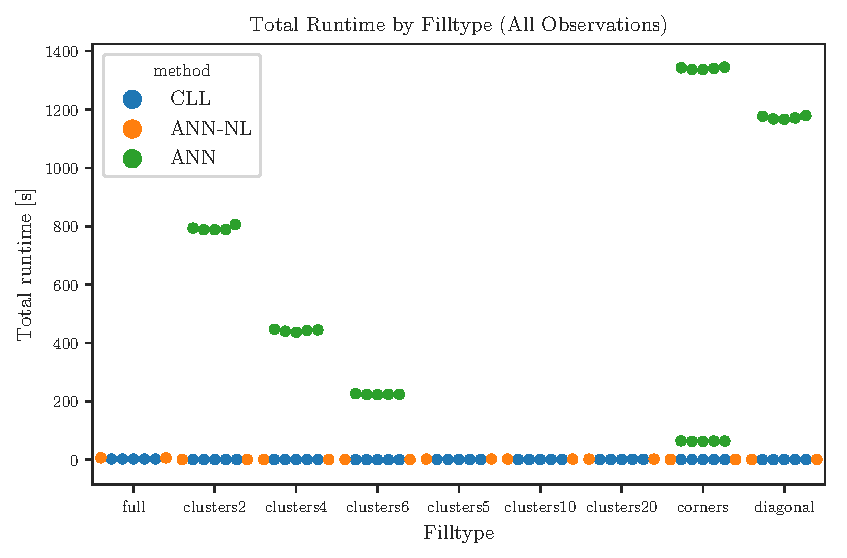
\includegraphics[width=\textwidth]{figures/totalruntime_all.pdf}
	\caption{FIXME!}
\end{figure}
\begin{figure}[h]
	\centering
	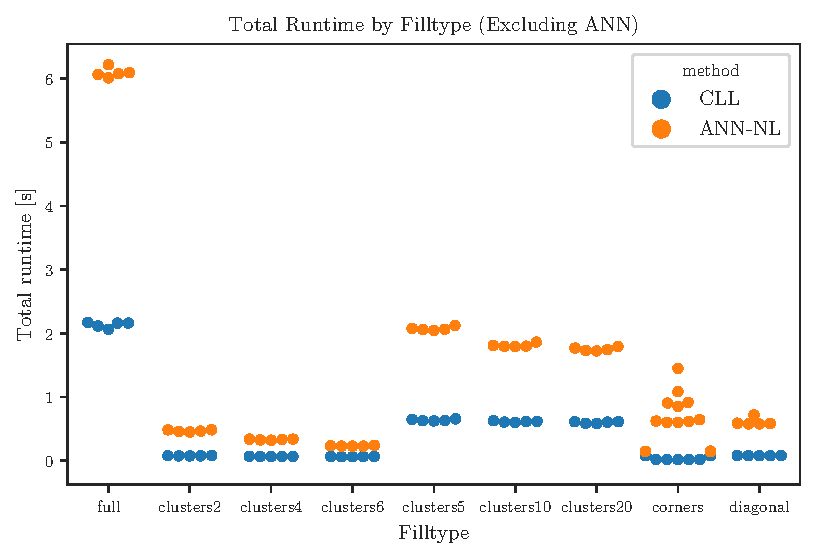
\includegraphics[width=\textwidth]{figures/totalruntime_noann.pdf}
	\caption{FIXME!}
\end{figure}



ann and list building in detail -> throw out

compare search times of ann and annnolist - compiler?

corners, compare across fills

11, compare across filltypes


Datenquelle nachvollziehbar und abgelegt

Einfüsse (Befüllungsgrad, Suche) einzelnd hervorheben


In diesem Kapitel werden die Ergebnisse beschrieben, diskutiert und ggf. mit anderen Daten aus der Literatur verglichen. Die Diskussion soll klären, ob die Daten sinnvoll sind, die Ergebnisse so zu erwarten waren und ob ungewöhnliche Beobachtungen sichtbar sind. Es ist auf eine übersichtliche Struktur zu achten, untersuchte Fälle sind konsistent und logisch zu benennen. Die Darstellung der Daten ist an die verwendete Messgenauigkeit anzupassen (z.B. ist eine Angabe von \SI{314.394575}{K} in den meisten Fällen nicht sinnvoll).
 
\chapter{Summary and Outlook}

Die Zusammenfassung ermöglicht Außenstehenden einen Überblick über den Inhalt der Arbeit und enthält insbesondere die Zielsetzung, die verwendete Methodik, Verfahren und Ansätze sowie die erzielten Ergebnisse. Daran schließt sich ein Ausblick an, der mögliche Verbesserungen bzw. weitere Arbeitsschritte aufzählt. Die Zusammenfassung ist das am häufigsten gelesene Kapitel (größt mögliche Sorgfalt!) und umfasst maximal zwei bis drei Seiten.



%% Auf ungerader Seite starten
\cleardoublepage
%%%%%%%%%%%%%%%%%%%%%%%%%%%%%%%%%%%%%%%%%%%%%%%%%%%%%%%%%%%%%%%%%%%%%%%%%%%%%%%%%%%%%%%%%
% Einleitung
%%%%%%%%%%%%%%%%%%%%%%%%%%%%%%%%%%%%%%%%%%%%%%%%%%%%%%%%%%%%%%%%%%%%%%%%%%%%%%%%%%%%%%%%%

\chapter{Abschlussarbeiten am ITS}
\label{Chapter:Aufbau der Arbeit}

Diese Vorlage dient zur Erstellung wissenschaftlicher Abschlussarbeiten am Institut für Thermische Strömungsmaschinen (ITS) und stellt eine Zusammenfassung der Meinungen aller wissenschaftlicher Mitarbeiter dar. Zu manchen Punkten kann der Betreuer eigene Meinungen haben. Es existiert eine äquivalente Word-Vorlage, deren Benutzung mit dem Betreuer abzusprechen ist. 

In diesem Kapitel wird auf den allgemeinen Aufbau einer Abschlussarbeit eingegangen. In Kapitel~\ref{CHAPTER:Hinweise} wird im Detail auf einzelne Aspekte der sprachlichen Gestaltung, Aufbau von Gliederung, Diagrammen, Abbildungen sowie Gleichungen eingegangen.

\section{Allgemeines}
Die Arbeit ist in deutscher Sprache anzufertigen und wird einseitig gedruckt. Der Gesamtumfang beträgt in der Regel für Bachelorarbeiten 30~--~60 und für Masterarbeiten 60~--~80 Seiten. Diese Angaben sind lediglich als Richtlinie zu werten und erfolgen immer in Absprache mit dem Betreuer. Vor Beginn des Schreibens ist die Gliederung mit dem Betreuer abzusprechen. Um den Korrekturaufwand möglichst gering zu halten, ist es sinnvoll, eine Vorkorrektur an einem Teil der Arbeit durchzuführen, bevor die gesamte Arbeit zur Korrektur abgegeben wird. Für die Einarbeitung in das Thema sollten ungefähr zwei Wochen eingeplant und spätestens sechs Wochen vor Abgabe mit dem Schreiben begonnen werden.

Grundsätzlicher Aufbau einer Abschlussarbeit:
\begin{itemize}
\itemsep0em 
	\item ITS Deckblatt
	\item Leerseite
	\item Gegebenenfalls ein Sperrvermerk
	\item Aufgabenstellung
	\item Unterschriebene eidesstattliche Erklärung
	\item Danksagung (freiwillig!)
	\item Evtl. Kurzfassung/Abstract
	\item Inhaltsverzeichnis
	\item Abbildungsverzeichnis
	\item Tabellenverzeichnis
	\item Symbolverzeichnis
	\item \textbf{Hauptteil} (siehe folgende Unterkapitel)
	\item Literaturverzeichnis
	\item Anhang
\end{itemize}

Im Folgenden ist beschrieben, aus welchen Bausteinen der Hauptteil einer Abschlussarbeit besteht, welche Aufgabe diese Bausteine haben und wie sie mit Inhalt zu füllen sind. Um den Leser an einem \glqq roten Faden\grqq~durch die Arbeit zu führen, ist es hilfreich kurze Zusammenfassungen am Ende der Kapitel bzw. Überleitungen zum nachfolgenden Kapitel zu liefern.

\section{Einleitung}
\label{SECTION:Einleitung}

Die Einleitung hat die Funktion zum Thema hinzuführen und liefert Antworten, warum das Thema der Arbeit aus technischer, wissenschaftlicher und evtl. wirtschaftlicher Sicht von Bedeutung ist. Mit Ende der Einleitung muss das Thema der Arbeit klar beschrieben sein. Daher ist der Anfang sehr allgemein gehalten, während zum Schluss das Problem eingegrenzt wird. Hier gilt: Möglichst keine externe Quellen!

\section{Stand der Forschung}

Im Stand der Forschung wird aufgezeigt, welche Arbeiten es zu diesem bzw. ähnlichen Themen gibt und welche Lücke diese Arbeit füllen soll. Hierbei sind vor allem sämtliche Vorgängerarbeiten des ITS ausfindig zu machen. Als Quellen sind bevorzugt Zeitschriftenartikel und Konferenzbeiträge statt Dissertationen anzugeben. Im letzten Abschnitt des Kapitels wird eine konkrete Zielsetzung der Arbeit und die Vorgehensweise erarbeitet.


\section{Grundlagen}

Grundlagen, die zum Verständnis der weiteren Kapitel notwendig sind, werden beschrieben. Daher ist dieses Kapitel möglichst knapp zu gestalten, es handelt sich nicht um ein Lehrbuch! Um Platz zu sparen, können Verweise auf weiterführende Lehrbücher verwendet werden. Zum Beispiel: 
\begin{quote}
	\glqq Im Rahmen dieser Arbeit kommt nur das $k\text{-}\epsilon$-Turbulenzmodell zum Einsatz. Deshalb wird an dieser Stelle auf andere Turbulenzmodelle nicht weiter eingegangen. Diese werden ausführlich in Autor XY et al. (2017) erläutert.\grqq
\end{quote}
Aussagen in diesem Kapitel werden mit Quellenangaben versehen, wenn es sich nicht um allgemeines Wissen im Ingenieurwesen handelt. Herleitungen komplexer Formeln sind nur mit Bedacht zu verwenden. Um zu verhindern, dass der Leser gezwungen ist im Text vor- und zurückzuspringen, ist auf einen logischen Aufbau des Kapitels zu achten. Dies kann zum Beispiel nach Teilgebieten, chronologisch oder nach Komplexität gestaltet sein. Verweise auf noch kommende Textstellen sind zu vermeiden. Besser: \glqq In Abschnitt \ref{SECTION:Einleitung} wurde gezeigt, dass ... \grqq.

\section{Material und Methoden}

Hier wird der experimentelle Aufbau bzw. das verwendete numerische Modell beschrieben und die Vorgehensweise der Arbeit dargelegt. Es soll kein Benutzerhandbuch zur eingesetzten Software enthalten! Die folgenden exemplarischen Gliederungen können als Orientierungshilfe dienen:

Beispiel für numerische Arbeit:
\begin{itemize}
\itemsep0em 
	\item Geometrie
	\item Netz
	\item Anfangs- und Randbedingungen
	\item Verwendete Solver, Zeitschrittweite, Konvergenzkriterien, ...
	\item Einlaufrechnung, Mitteilungsdauer, ...
\end{itemize}

Beispiel für experimentelle Arbeit:
\begin{itemize}
\itemsep0em 
	\item Versuchsaufbau und Geometrie
	\item Eingesetzte Messtechnik
	\item Angabe der Messgenauigkeit
	\item Vorgehensweise bei der Versuchsdurchführung
\end{itemize}

\section{Ergebnisse und Diskussion}

In diesem Kapitel werden die Ergebnisse beschrieben, diskutiert und ggf. mit anderen Daten aus der Literatur verglichen. Die Diskussion soll klären, ob die Daten sinnvoll sind, die Ergebnisse so zu erwarten waren und ob ungewöhnliche Beobachtungen sichtbar sind. Es ist auf eine übersichtliche Struktur zu achten, untersuchte Fälle sind konsistent und logisch zu benennen. Die Darstellung der Daten ist an die verwendete Messgenauigkeit anzupassen (z.B. ist eine Angabe von \SI{314.394575}{K} in den meisten Fällen nicht sinnvoll).

\section{Zusammenfassung und Ausblick}

Die Zusammenfassung ermöglicht Außenstehenden einen Überblick über den Inhalt der Arbeit und enthält insbesondere die Zielsetzung, die verwendete Methodik, Verfahren und Ansätze sowie die erzielten Ergebnisse. Daran schließt sich ein Ausblick an, der mögliche Verbesserungen bzw. weitere Arbeitsschritte aufzählt. Die Zusammenfassung ist das am häufigsten gelesene Kapitel (größt mögliche Sorgfalt!) und umfasst maximal zwei bis drei Seiten.

\section{Anhang}

Stören umfangreiche Ergebnisse oder Daten den Lesefluss, werden sie nur auszugsweise in den Kern der Arbeit übernommen. Der Rest kommt in den Anhang. Programmcode kommt nach Absprache mit dem Betreuer auch in den Anhang. Aktive Verweise auf den Anhang sind zu vermeiden. Nicht: \glqq In Abbildung A.12 ist eine Skizze des Versuchsaufbaus dargestellt. Die Probe ist unterhalb des Messkopfes eingespannt und ... \grqq. In diesem Fall ist die Abbildung zu wichtig für den Anhang und wird stattdessen besser im entsprechenden Kapitel platziert.
%\input{kapitel/TeXintro.tex}
%% Auf ungerader Seite starten
\cleardoublepage
%%%%%%%%%%%%%%%%%%%%%%%%%%%%%%%%%%%%%%%%%%%%%%%%%%%%%%%%%%%%%%%%%%%%%%%%%%%%%%%%%%%%%%%%%
% Zielsetzung und Vorgehensweise
%%%%%%%%%%%%%%%%%%%%%%%%%%%%%%%%%%%%%%%%%%%%%%%%%%%%%%%%%%%%%%%%%%%%%%%%%%%%%%%%%%%%%%%%%

\chapter{Weitere Hinweise}
\label{CHAPTER:Hinweise}

In diesem Kapitel wird auf einzelne Aspekte im Detail eingegangen. Zunächst wird die sprachliche Gestaltung behandelt, im weiteren Verlauf der Aufbau der Gliederung. Schließlich werden einige Besonderheiten zu Diagrammen, Abbildungen sowie Gleichungen erläutert.
\section{Sprachliche Gestaltung}
\label{SECTION:Sprache}

Das Ziel einer Abschlussarbeit ist, den untersuchten Sachverhalt möglichst einfach und leicht verständlich darzustellen. Komplizierte Satz- bzw. Wortstrukturen, die den Leser beeindrucken sollen, haben hier nichts zu suchen. Es ist sprachlich zwischen Gegenständen, beobachtbaren physikalischen Phänomenen, messbaren physikalische Größen und dem Wert der physikalischen Größen zu unterscheiden. Eine korrekte Formulierung ist beispielsweise: 
\begin{quote}
	\glqq Es findet Wärmeübertragung vom Fluid auf die Rohrleitung statt. Die Leitung ändert daher ihre Temperatur. Diese beträgt \SI{815}{\celsius}\grqq.
\end{quote}

Falsch ist hingegen: 

\begin{quote}
	\glqq Die Leitung hat \SI{815}{\celsius}\grqq~oder \glqq Die Wärmeübertragung wurde gemessen\grqq~und niemals: \glqq Die Leitung wurde gemessen\grqq.
\end{quote}

Ein Gegenstand hat genau einen Namen. Synonyme sind zu vermeiden, falls nicht völlig klar ist, dass mit beiden Begriffen dasselbe gemeint ist. Es sind aussagekräftige und eindeutige Beschreibungen zu verwenden. Zum Beispiel können Begriffe wie stromauf oder stromab eine eindeutigere Beschreibung liefern als horizontal oder vertikal. Auch rechts oder links sowie oben oder unten werden besser durch funktionsbezogene Lagebezeichnungen ersetzt. Beispielsweise: 

\begin{quote}
	\glqq Der Wirbel befindet sich stromab der rückspringenden Stufe im Strömungskanal. Zur Messung des Geschwindigkeitsfeldes im Wirbel wird eine Sonde quer zur Strömungsrichtung traversiert.\grqq
\end{quote}

Sätze, die sich über mehr als drei Zeilen erstrecken, stören den Lesefluss und werden besser in einzelne Sätze unterteilt. Zur Strukturierung von Sätzen zu Gedanken können Absätze eingesetzt werden. Sätze werden im Passiv konstruiert (kein \glqq man\grqq, \glqq ich\grqq, \glqq wir\grqq). Füllwörter, wie z.B. \glqq jedoch, hierfür, ...\grqq, sind zu vermeiden. Diese beinhalten keine Information und sind daher nicht notwendig. Lange Listen oder Aufzählungen sind ebenfalls zu vermeiden.

Eine korrekte Rechtschreibung und Interpunktion ist verpflichtend (Rechtschreibreform vom August 2006). Daher immer ein Rechtschreibprogramm nutzen! Als Dezimaltrennzeichen wird das Komma verwendet (\SI{1,3} {\km}). Bis auf Vorgehensweise und Zusammenfassung werden alle Kapitel im Präsens verfasst.

\section{Gliederung}
\label{SECTION:Gliederung}

\subsection{überflüssige Überschrift}

Auf einen Punkt x.y.1. folgt immer ein Punkt x.y.2. Wenn nicht, so ist der Punkt x.y.1 unnötig. Die Untergliederung auf der nächst höheren Ebene ist dann ausreichend. Empfehlung: Nach einer Kapitel- (Abschnitts-)Überschrift folgt i.d.R. Text und nicht etwa eine weitere Überschrift oder eine Abbildung. Gliedert sich das Kapitel X in X.1 und X.2, so könnte zu Beginn das Kapitels X z.B. stehen, was im Kap. X besprochen werden soll und wie sich dies auf die Unterkapitel aufteilt, warum die Themen des Kapitels X wichtig sind oder/und wie diese Themen mit dem Rest der Arbeit zusammenhängen. Die Gliederung ist so zu strukturieren, dass sie nicht mehr als drei Unterebenen (3.2.1, 3.2.1.1) enthält, vor allem nicht im Inhaltsverzeichnis. Treffende Überschriften wählen. Nicht \glqq Messaufbau\grqq, sondern \glqq Laseroptische Methode zur Untersuchung des Streuverhaltens\grqq.


\section{Literaturverweise}
\label{SECTION:Literaturverweise}

Alle zur Durchführung der Arbeit und zu deren Nutzen herangezogenen Quellen sind im Text zu beschreiben oder zumindest zu erwähnen und in einem Literaturverzeichnis am Ende des Hauptdokumentes aufzulisten. Außerdem sollten sie dem Betreuer in einer geeigneten Form verfügbar gemacht werden. Ist eine Quelle nur schwierig oder kurz verfügbar (z.B. weil ein Buch nur für kurze Zeit ausgeliehen werden darf), so ist eine Kopie der für die Arbeit wesentlichen Passagen anzufertigen. Internetquellen (auch Wikipedia) sind nicht als seriöse Quelle geeignet und mit adäquaten Fachliteraturquellen zu ersetzen. Falls die Angabe im Ausnahmefall notwendig ist, wird die Quelle in Form einer html-Datei oder eines Screenshots festgehalten. Direkte Zitate der Form:
\begin{quote}
	„In modernen Hochleistungstriebwerken betragen die Kühlluftmassenströme bereits über 30\% des gesamten Massenstroms der Kernmaschine.“ (\cite{baldauf2001}),
\end{quote}


sind zu vermeiden.

\nocite{*} % Alle Quellen werden im Quellenverzeichnis genannt, auch wenn Sie im Text nicht referenziert werden.

% Die folgenden Befehle helfen den Zitierstil gegebenenfalls anzupassen:
%\begin{tabbing}
%	\cite{baldauf2001,kneer2015}\\
%	\citep[s.a.][]{baldauf2001,kneer2015}\\
%	\citet{baldauf2001,kneer2015}\\
%	\\
%	\cite{winklhofer91,kneer2015}\\
%	\citep{winklhofer91,kneer2015}\\
%	\citet{winklhofer91,kneer2015}\\
%	\\
%	\cite{kneer2015}\\
%	\citep{kneer2015}\\
%	\citet{kneer2015}\\
%	\citet*{kneer2015}\\
%	\citeauthor{kneer2015}\\
%	\citeauthor*{kneer2015}\\
%	\citeyear{kneer2015}\\
%	\citeyearpar{kneer2015}\\
%	\\
%	\cite{winklhofer91}\\
%	\citep{winklhofer91}\\
%	\citet{winklhofer91}\\
%	\citet*{winklhofer91}\\
%	\citeauthor{winklhofer91}\\
%	\citeauthor*{winklhofer91}\\
%	\citeyear{winklhofer91}\\
%	\citeyearpar{winklhofer91}\\
%\end{tabbing}

\section{Abbildungen und Tabellen}
\label{SECTION:Abbildungen}

Abbildungen werden im Text erläutert: Abbildung~\ref{GRAPHIC:DomainKeller} lassen sich die physikalischen und geometrischen Eigenschaften des berechneten Gebiets entnehmen. Daher ist die Abbildung so platziert, dass sie nach dem Text erscheint, in dem diese beschrieben werden. Ebenso wird die Aussage der Abbildung erläutert: Die Fluid begrenzenden Flächen sind blau dargestellt, ... . Passiv konstruieren: Nicht \glqq Das Bild 2.4 zeigt\grqq, sondern \glqq In Bild 2.4 ist gezeigt\grqq. 

%Diese Abbildung wurde mit Inkscape erstellt, sodass die Grafik als pdf vorliegt, der Text aber in einer tex-Datei.

\begin{figure}[h]
	\centering
	\def\svgwidth{0.6\columnwidth}
	%\input{bilder/keller_2016.pdf_tex}	
	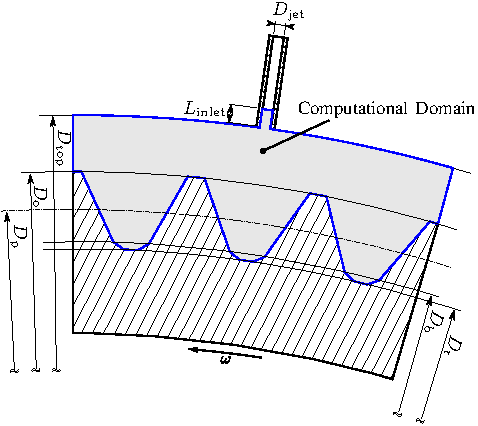
\includegraphics[width=0.7\textwidth]{bilder/keller_2016.pdf}
	\caption{Querschnitt durch das berechnete Segment des Zahnrads, \cite{keller2016}}
	\label{GRAPHIC:DomainKeller}
\end{figure}

% Die Platzierung der Abbildungen in figure-Umgebung kann anhand Optionen gesteuert werden:
% h - Die Abbildung wird wenn möglich an der Stelle der Definition eingefügt
% t - Die Abbildung wird oben auf der Seite platziert
% b - Die Abbildung wird unten auf der Seite platziert
% p - Eine eigene Seite mit Abbildungen wird angelegt
% Die Angabe von \begin{figure}[htbp] gibt die Priorität an. Zuerst wird versucht die Grafik an Ort und Stelle zu erzeugen. Gelingt dies nicht wird sie oben auf der Seite eingefügt, usw.

% Per \subcaptionbox können Abbildungen nebeneinander platziert und mit a), b) beschriftet werden
%\begin{figure}[ht]
%	\centering
%	\subcaptionbox{}{\includegraphics[width=0.48\columnwidth]{bilder/Bild_1_von_2}}\hfill
%	\subcaptionbox{}{\includegraphics[width=0.48\columnwidth]{bilder/Bild_2_von_2}}
%	\caption{GRAPHICS PLACED SIDE BY SIDE AND AMONG EACH OTHER WITH SUBORDINATE CAPTIONS}
%	\label{figure:_several_graphics}
%\end{figure}

Abbildungen helfen dem Autor, seine Erkenntnisse zu erläutern oder zu belegen. Diese Verbindung zwischen Abbildung und Aussage muss deutlich werden, sonst ist die Abbildung zu streichen. Alle Grafiken, Abbildungen und Tabellen müssen im Text referenziert und besprochen werden. Die Referenz ist durch eine fortlaufende Nummerierung der Objekte eindeutig vorzunehmen. Dabei werden Objekte gleichen Typs wie z.B. Abbildungen, Gleichungen und Tabellen jeweils gesondert nummeriert. Auf ein einheitliches Erscheinungsbild und Lesbarkeit achten (Textgröße, Auflösung, Größe angepasst an DIN A4, Vektorgrafiken wenn möglich). Abbildungen, die nicht selbst erstellt wurden, müssen ebenfalls zitiert werden. Wenn sie verändert wurden: \glqq Abbildung nach \cite{schoof2014}\grqq. Im Gegensatz zu Abbildungen besitzen Tabellen keine Unter- sondern Überschriften (siehe Tabelle \ref{tab:experiment-parameters}). Die Unterschriften sind möglichst aussagekräftig und eindeutig zu gestalten. Weitere Tabellenbeispiele werden von Markus Püschel\footnote{\url{https://www.inf.ethz.ch/personal/markusp/teaching/guides/guide-tables.pdf}} aufgezeigt. 

% Simple Beispiel-Tabelle
%\begin{table}[h]
%	\centering
%	\captionabove{Eine sinnlose Tabelle}
%	\begin{tabular}{|c|c|c|}
%		\hline
%		Spalte 1 & Spalte 2 & Spalte 3 \\
%		\hline
%		1 & 2 & 3 \\
%		\hlin den Diagrammen vergleichbar sein sollen (siehe Abbildung~\ref{fig:several_graphics}). Eventuell ist auch eine logarithmische Auftragung sinnvoll. Diagramme besitzen eine Legende. Sinnvolle min./max. Werte festlegen (nicht 0,2845 bis 9,385, sondern besser 0 bis 10). Ein Raster (\glqq grid\grqq) kann hilfreich sein. Diagramme farblich so gestalten, dass sie auch in schwarzweiß lesbar sind. In Abbildung \ref{fig:several_graphics} sind neben der farblichen Gestaltung zusätzlich unterschiedliche Marker und Linienarten eingesetzt. In der Regel ist der Hintergrund weiß, Sonderformatierungen (Hintergründe, Schriftarten) sind nur einzusetzen, wenn Vorteile daraus entstehen. Bei der Farbgebung auf die Erscheinungsform achten, zum Beispiel unterscheidet sich die Darstellung auf dem Beamer von der einer schriftlichen Ausarbeitung. Diagramme besitzen keinen alles umschließenden Rahmen. Abbildung möglichst einfach und leicht verständlich gestalten, in der Regel nicht mehr als drei Linien im Diagramm.

\begin{figure}[htpb]
	\centering
	\subcaptionbox{$x = \SI{0,7}{\mm}$} {\includeraphics[width=0.48\columnwidth]{bilder/wieth_2016_2_6}}\hfill
	\subcaptionbox{$x = \SI{1,0}{\mm}$}{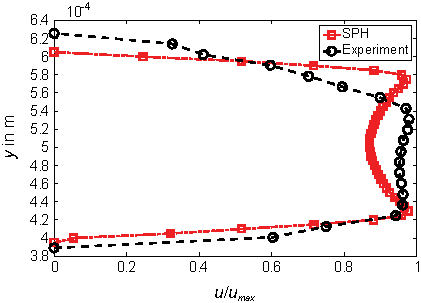
\includegraphics[width=0.48\columnwidth]{bilder/wieth_2016_2_6}}
	\subcaptionbox{$x = \SI{1,1}{\mm}$} {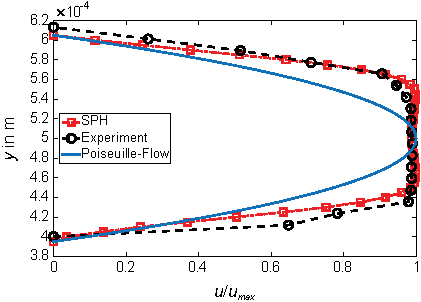
\includegraphics[width=0.48\columnwidth]{bilder/wieth_2016_3_6}}\hfill
	\subcaptionbox{$x = \SI{2.0}{\mm}$}{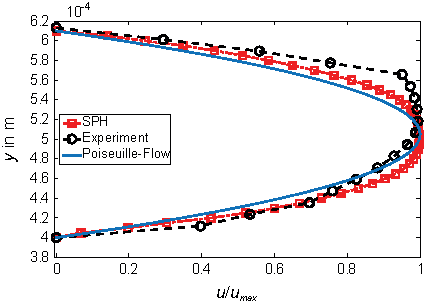
\includegraphics[width=0.48\columnwidth]{bilder/wieth_2016_4_6}}
	\subcaptionbox{$x = \SI{2,5}{\mm}$} {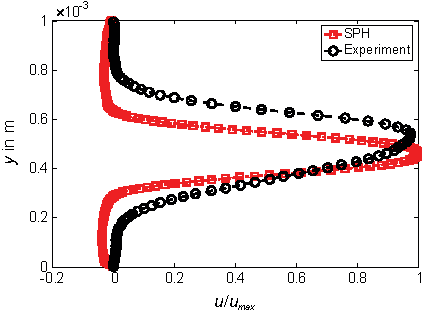
\includegraphics[width=0.48\columnwidth,height=5.5cm]{bilder/wieth_2016_5_6}}\hfill
	\subcaptionbox{$x = \SI{3,0}{\mm}$}{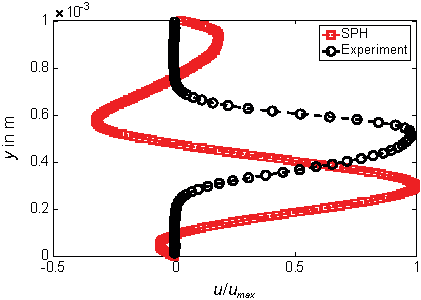
\includegraphics[width=0.48\columnwidth, height=5.5cm]{bilder/wieth_2016_6_6}}
	\caption{Vergleich zwischen experimentellen (kreisförmig) und berechneten (quadratisch) Werten, modifiziert nach \cite{wieth2016}. Da die Diagramme aus einer englischen Veröffentlichung stammen, sind die Dezimaltrennzeichen fälschlicherweise Punkte}
	\label{fig:several_graphics}
\end{figure}

\clearpage

\section{Gleichungen}
\label{SECTION:Gleichungen}

Alle Formelzeichen, die in einer Gleichung auftreten und nicht schon im vorangehenden Text definiert wurden, sind zu benennen und zu erläutern. In der Literatur etablierte Formelzeichen zur Beschreibung von physikalischen Größen wählen. Ein Formelzeichen beschreibt genau eine physikalische Größe. Jede physikalische Größe wird mit genau einem Formelzeichen beschrieben. Der Übersichtlichkeit halber mit Indizes und eingängigen Namen arbeiten. Gleichungen werden zentriert, nummeriert und sind Teil eines Satzes (besitzen also Satzzeichen). Zum Beispiel beschreibt der Impulssatz der Strömungsmechanik,

\begin{equation}
\label{EQUATION:Impuls}
\sum\vec{F}=\frac{d\vec{I}}{dt}=\underbrace{\frac{\partial}{\partial t}\iiint\varrho\:\vec{w}\:dV}_{\text{instationär}} + \underbrace{\iint\varrho\:\vec{w}\:\left(\vec{w}\cdot\vec{n}\right)\:dA}_{\text{stationär}},
\end{equation}

die zeitliche Änderung des Impulses $\frac{d\vec{I}}{dt}$ innerhalb eines Kontrollvolumens $V$, mit  der Dichte $\varrho$, dem Geschwindigkeitsvektor $\vec{w}$, der Oberfläche $A$ und dem äußeren Oberflächennormalen-Einheitsvektor $\vec{n}$. Die Änderung des Impulses entspricht der Summe der äußeren Kräfte $\sum\vec{F}$.

Formelzeichen werden immer zusammen mit einer Bezeichnung erwähnt. Die Angabe des Werts einer physikalischen Größe erfolgt immer mit der entsprechenden Einheit:

\begin{quote}
	$\Delta T$ = \SI{452,69}{\kelvin}.
\end{quote}

Zwischen Größe und Einheit, wie \SI{2,0}{\mm}, wird ein halbes Leerzeichen gesetzt (umbruchgeschütztes Leerzeichen verwenden bzw. \LaTeX-Paket siunitx). Einheiten und Operatoren, wie \glqq log\grqq, werden nicht kursiv gesetzt. Innerhalb der Arbeit auf eine einheitliche Darstellung für Vektoren, Tensoren etc. achten und SI-Einheiten verwenden.

%Formeln über mehrere Zeilen können zum Beispiel so realisiert werden:
%\begin{eqnarray}
%\sigma_e & = & n_0 \pi r^2 \xi_e \nonumber \\
%\sigma_s & = & n_0 \pi r^2 \xi_s \\
%\sigma_a & = & \sigma_e - \sigma_a
%\end{eqnarray}
% & richtet die einzelnen Zeilen zueinander aus.

%\section {Some text}
%TeX does not mean only programing and using commands. Examining the source-code of the text below, you will realise that typing a bigger paragraph of text is relatively simple and does not require more effort for formatting than with other programs. In the text-section below, among other things, some examples for font formatting and referencing are given.
%
%Fig.~\ref{figure:_zeilenumbruch} shows selected results of the LDV measurements of the gaseous 
%phase. In the upper diagram the phase averaged temporal 
%variation of the vertical component (axial velocity) 
%$u_{G,Y}(\phi)=\overline{u}_{G,Y}+u'_{G,Y}(\phi)$ is presented for a pulsating gaseous flow at a constant excitation 
%frequency of $f_S=\SI{250}{Hz}$, different mean velocities $\overline{u}_G$ and a constant 
%bypass setting of the siren. Apparently, the instantaneous 
%velocity $u_{G,Y}(\phi)$ is increasing with the mean velocity $\overline{u}_G$. However, the 
%relation is not proportional. There is a loss of velocity due to the positioning of the 
%LDV measuring volume in the wake of the prefilming surface and the divergence of the open jet. 
%Furthermore, the phase shift 
%is moving towards an earlier time at higher mean velocities. This can be explained by 
%the longer wavelength $\lambda \approx \overline{u}_G/f_S$ of the convected pulsation.
%It has to be noted that the signals are not perfectly sinusoidal 
%as anticipated. The fundamental mode is superimposed by a 
%first and second harmonic oscillations and additional noise. However, 
%those perturbing components represent only a fraction of the 
%designated signal.


%%%%%%%%%%%%%%%%%%%%%%%%%%%%%%%%%%%%%%%%%%%%%%%%%%%%%%%%%%%%%%%%%%%%%%%
% Literaturverzeichnis und Anhang
%%%%%%%%%%%%%%%%%%%%%%%%%%%%%%%%%%%%%%%%%%%%%%%%%%%%%%%%%%%%%%%%%%%%%%%
% Literaturverzeichnis auf einer ungeraden (rechten) Seite starten !
\cleardoublepage
%%%%%%%%%%%%%%%%%%%%%%%%%%%%%%%%%%%%%%%%%%%%%%%%%%%%%%%%%%%%%%%%%%%%%%
%  Literaturverzeichnis
%%%%%%%%%%%%%%%%%%%%%%%%%%%%%%%%%%%%%%%%%%%%%%%%%%%%%%%%%%%%%%%%%%%%%%
\refstepcounter{dummy}
\addcontentsline{toc}{chapter}{\refname}
%% Verschiedene Zitationsstile
% ITS
\bibliographystyle{literatur/itsBibStyle}
% Sonstige
%\bibliographystyle{plaindin}
%\bibliographystyle{unsrtdin}
%\bibliographystyle{abbrvdin}
%\bibliographystyle{alphadin}

%%%%%%%%%%%%%%%%%%%%%%%%%%%%%%%%%%%%%%%%%%%%%%%%%%%%%%%%%%%%%%%%%%%%%%
\bibliography{literatur/beispiel}

%% Auf ungerader Seite starten
\cleardoublepage
%%%%%%%%%%%%%%%%%%%%%%%%%%%%%%%%%%%%%%%%%%%%%%%%%%%%%%%%%%%%%%%%
% Anhang
%%%%%%%%%%%%%%%%%%%%%%%%%%%%%%%%%%%%%%%%%%%%%%%%%%%%%%%%%%%%%%%%
\appendix
\chapter*{\appendixname}
\stepcounter{chapter}
\addcontentsline{toc}{chapter}{\appendixname}		% Name des Anhangs in Inhaltverzeichnis auf Kapitelebene schreiben
\ihead{\appendixname}								% Kopfzeile setzen

%%%%%%%%%%%%%%%%%%%%%%%%%%%%%%%%%%%%%%%%%%%%%%%%%%%%%%%%%%%%%%%%
\section{Anhang 1}
\begin{table}[htbp]
	\centering
	\renewcommand{\arraystretch}{1.3} % Größerer Zeilenabstand
	\captionabove{Simulationsergebnisse, die den Lesefluss stören.}
	\begin{tabular}{@{}rrrrcrrr@{}}
		\toprule
		&\multicolumn{3}{c}{$w = 8$} & \phantom{abc}& \multicolumn{3}{c}{$w = 16$}  \\
		\cmidrule{2-4} \cmidrule{6-8}
		& $t=0$ & $t=1$ & $t=2$ && $t=0$ & $t=1$ & $t=2$  \\
		\midrule
		$dir=1$ \\
		$c$ & 0,0790 & 0,1692 & 0,2945 && 0,3670 & 0,7187 & 3,1815 \\
		$c$ &  -0,8651& 50,0476& 5,9384&& -9,0714& 297,0923& 46,2143\\
		$c$ & 124,2756& -50,9612& -14,2721&& 128,2265& -630,5455& -381,0930\\
		$dir=0$\\
		$c$ & 0,0357& 1,2473& 0,2119&& 0,3593& -0,2755& 2,1764\\
		$c$ & -17,9048& -37,1111& 8,8591&& -30,7381& -9,5952& -3,0000\\
		$c$ & 105,5518& 232,1160& -94,7351&& 100,2497& 141,2778& -259,7326\\
		\bottomrule
	\end{tabular}
	\label{tab:example-table}
\end{table}
\section{Anhang 2}
\lipsum

\end{document}
